\documentclass[12pt, a4paper,twoside]{tesi_upf}


\usepackage[latin1]{inputenc}
\usepackage[T1]{fontenc}


%IDIOMES
\usepackage[english,spanish]{babel}
\usepackage[cam,a4,center,frame]{crop}
\usepackage[colorlinks=false]{hyperref}
\usepackage{graphicx}
\usepackage{mathtools}
\usepackage{csquotes}
\usepackage{times}
\pagestyle{plain}
\usepackage[backend=biber,backref,url=false,bibencoding=utf8,sorting=none]{biblatex}
\usepackage{biblatex}
\usepackage{makeidx}
\usepackage{subcaption}
\usepackage{enumitem}
\usepackage{url}
\usepackage{tabularx}
\usepackage{adjustbox}
\usepackage{tabu}
\usepackage{mathtools}
\usepackage{tabulary}

\usepackage[newcommands]{ragged2e}
\newcommand\tr{\rule{0pt}{3.5ex}}
\newcommand\br{\rule[-3ex]{0pt}{3ex}}
\makeindex


%\bibliographystyle{apalike}
\setlength{\parindent}{1em}
\setlength{\parskip}{1em}



\selectlanguage{english}


\addto\captionscatalan
  {\renewcommand{\contentsname}{\Large \sffamily Sumari}}
\addbibresource{../bibliography/bibliography_tesis.bib}
\addbibresource{../bibliography/library.bib}


\title{El titulo de la tesi: In-silico methods to drug discovery}
\subtitle{El subtitulo de la tesi: Cancer}
\author{Autor: Francisco Mart\'inez Jim\'enez}
\thyear{L'any de la tesi: 2016}
\department{Departament: Biomedicine}
\supervisor{Director: Marc A. Marti-Renom}


\begin{document}

\frontmatter


\maketitle

\cleardoublepage




\noindent A mi madre. 

\cleardoublepage





\noindent {\Large \sffamily Agradecimientos} Agraeixo....

\cleardoublepage

\selectlanguage{english}
\section*{\Large \sffamily Abstract}
This is the abstract of the thesis in English.  Please, use less
than 150 words.

\selectlanguage{spanish}
\vspace*{\fill}
\section*{\Large \sffamily  Resum}

Vet aqui el resum de la tesi en catala.  
\vspace*{\fill}
\selectlanguage{english}
\cleardoublepage


%PREFACI OPCIONAL. SI NO ES VOL, COMENTEU FINS EL FINAL DE PREFACI
{\bf Prefaci}

\cleardoublepage
%FINAL DE PREFACI



\tableofcontents


\listoffigures

\addcontentsline{toc}{chapter}{Index of figures}


\listoftables

\addcontentsline{toc}{chapter}{List of tables}


\mainmatter

\chapter*{Summary}

sencillo

Consta de
\begin{description}
\item[tesi-upf.cls]{\tt book} 
  \begin{enumerate}
  \item Es redissenya la portada  \verb+\maketitle+).

  \item 

  \item Es redefineix {\tt cleardoublepage} para que las paginas en blanco no se numeren
  \end{enumerate}

\item[Preambulel] 
 

\item[paquets] {\tt crop} i {\tt geometry}. 




\item[Taules] Includes \verb+figure+ i un \verb+tabular+ 

\end{description}


\section*{Index}


\begin{enumerate}
\item lo llamas en preambulo  \verb+\usepackage{makeidx} \makeindex+ con esto lo imprimes \verb+\printindex+ con esto lo creas  \verb+makeindex+ 
\end{enumerate}



\chapter{Introduction} \label{introduction} 

\section{Protein are essential molecules}




\par The importance of proteins in biological chemistry is just reflected by their name, derived from the Greek word \textit{proteios}, and that means "of the first rank"\footnote{The term protein was coined by Jons Jacob Berzelius in 1838. It was first used by Gerardus Johannes Mulder, advised by Berzelius, in its publication  \textit{Bulletin des Sciences Physiques et Naturelles en N\'eerlande (1838). pg 104. SUR LA COMPOSITION DE QUELQUES SUBSTANCES ANIMALES}, where he observed that all proteins seemed to have the same empirical formula and came out to the erroneous idea that they might be composed of a single type of very large molecule. Berzelius proposed the name because the material seemed to be the primitive substance of animal nutrition that plants prepare for herbivores.}. Their presence is so essential that they  constitute most of the cell dry mass \cite{kessel2010}. They are not only the cell's building blocks, but also they perform nearly all the cell's functions. Some roles of proteins include serving as structural components of cells and tissues (e.g., \textit{keratin} or \textit{collagen}), transmission of information between cells by hormones such as the \textit{insulin} or the \textit{oxytocin}, facilitating the transport and storage of small molecules (e.g., the transport of oxygen by \textit{hemoglobin}) or providing a defense against foreign invaders (e.g., antibodies). Other proteins such as the \textit{actin} and the \textit{myosin} are responsible of muscle contraction and therefore our movement. However, the most fundamental role of proteins is their ability to act as enzymes, which, catalyzes most of the chemical reactions in biological systems. In summary, proteins are crucial macromolecules present in most of the processes carried out by the cell and, in spite of being extensively studied for many years, they still carry many unanswered questions.    
%\par There is experimental evidence of more than 30,000 human protein products derived from over 17,000 human genes \cite{human2014}. That means that each gene expresses on average nearly two different protein \textit{isoforms}.  However, not all the proteome is simultaneously expressed. Estimates say that there are between 8,000 and 9,000 genes expressed in all tissues (i.e. the housekeeping proteome)   

\subsection{Protein structure}

\par A protein is a molecule made from a long chain of amino acids linked thorough a covalent peptide bond. Proteins are therefore also known as \textit{polypeptides}. Attached to this repetitive chain are those portions of the amino acids that are not involved in the covalent bond, the \textbf{side chains}. Side chains confer the different physico-chemical properties of each of the 20 types of amino acids \cite{thecell2008}. The composition of the amino acid sequence determines the function and the structure of a protein. That is because the unique sequence creates a specific pattern of attractive and repulsive forces between amino acids along the polypeptide that leads to a folding process resulting in a specific three-dimensional structure. These forces are usually non-covalent  interactions between the side chains of the amino acids. Non-covalent interactions are weaker than covalent ones, allowing the folded structure to certain degree of  conformation mobility i.e: to be dynamic. This phenomenon is really important to facilitate the interaction with other molecules as we will explore further in \ref{ligand_intect}.  
\par Protein structures are complex conformation of atoms organized in a hierarchical manner \ref{fig:hierarchy_figure}. The first level of this hierarchy, referred to as the \textbf{primary structure}, is the ordered sequence of amino acids of the polypeptide. Certain segments of these chains, tend to form simple shapes such as helices, strands, turns or loops.  These folding patterns are referred to as secondary elements and collectively constitute the \textbf{secondary structure} of the protein. The two most frequent type of secondary elements are the $\alpha$-helixes and the $\beta$-sheets \cite{DSSP}. The overall chain tends to fold further into a three-dimensional  \textbf{tertiary structure}. Contrary to the secondary structure, the tertiary structure folding is driven by interactions from amino acids far apart in the primary sequence. The tertiary structure, is generally the most stable form of the protein, that is, the one that minimizes its free energy \cite{Dill1990}. Furthermore, the tertiary structure is also the biologically active form of the protein, and its unfolding usually leads towards partial o total inactivation of the protein. Finally, some proteins are composed by multiple folded chains. In such cases, each folded subunit folds independently and then joins the others forming a biologically active complex. This type of organization is considered as the \textbf{quaternary structure}.
\begin{figure}[h]

  \centering
  	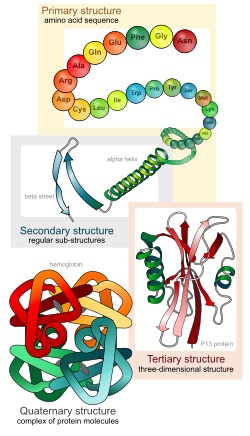
\includegraphics[scale=0.75]{../figures/protein_structure_levels_en.png} % Figure was taking from...

	\caption{Hierarchical distribution of layers in protein structure}
	\label{fig:hierarchy_figure}
\end{figure}
\par This traditional paradigm of protein structure has been challenged by some exceptions of proteins that lacks of a fixed or ordered three-dimensional structure. The intrinsically disordered proteins (IDPs) cover a wide spectrum of states from fully unstructured to partially structured including conformations such as \textit{random coils} or \textit{molten globules}. Moreover, some  factors may lead to the permanent loss of structure of a protein, and when that occurs, they endanger the entire organism. How problematic protein misfolding can be for the organism is illustrated by examples such as cystic fibrosis, Alzheimer's, Parkinson's and Huntington's diseases.
\par Figure \ref{fig:strucrure_sequence_figure} from the seminal paper \cite{StructureSequence} shows the correlation degree to which protein structures changed as a function of sequence divergence. This work helped to set up the fundaments of what is considered a central paradigm in protein evolution: protein structure is more conserved than sequence. However, not all the regions in a protein structure are equally conserved. It's been shown that functionally important amino acids, responsible of the interaction with other molecules, are more conserved than the rest of the protein structure \cite{conservPPI}. Additionally, the structural core is more conserved than the surface \cite{Raj2007}. The high conservation of the core enables the protein to maintain the global shape, while the surface is free to change (i.e.to mutate) some functional features \cite{Todd2001}.   These evolutionary mechanism are in accordance with the central \textit{sequence $\rightarrow$ structure $\rightarrow$ function} paradigm that prevails in the protein evolution field. 

\begin{figure}[h]

  \centering
  	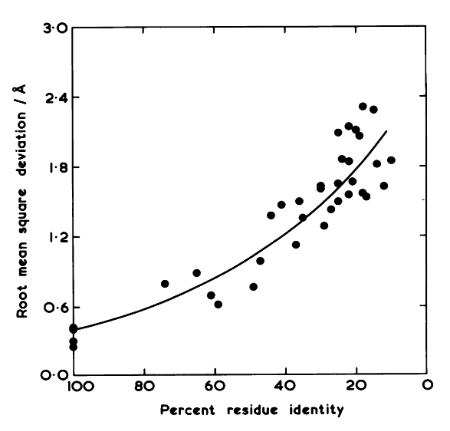
\includegraphics[scale=0.5]{../figures/structure_vs_sequence.png} % Figure was taking from...

	\caption{The original plot of the relation of residue identity and the r.m.s. deviation of the backbone atoms of the common cores of 32 pairs of homologous proteins. Figure extracted from \cite{StructureSequence}}
	\label{fig:strucrure_sequence_figure}
\end{figure}
 
\subsubsection{Protein Structure Determination}

\par Since in 1960, the Brithis biochemist John Kendrew determined the myoblobin structure \cite{KENDREW1960}, more than 37,000 different protein structures have been deposited in the Protein Data Bank (PDB) \cite{Berman2000}. The PDB is a repository created in the 1970s with the aim of storing all the 3D protein structures and unifying their format. Figure \ref{fig:structures_pdb} shows the variation of the number of deposited structures over the time. The number of PDB structures has significantly been increased over the last years thanks to initiatives such as the Protein Structure Initiative (PSI) \cite{Norvell2007} or the structural genomics \cite{GIleadi2007}. The later, was born with the aim of determining the structure of all human proteins. However, soon after, they realized that the goal was unrealistic. Fortunately, the number of folds which represent the complete \textit{fold space} observed in nature is much smaller that the number of proteins. Therefore, the current goal is to determine the structure of a representative set of proteins, that is, at least one protein per fold class. Once It is known the structure of one representative protein, and thanks to the \textit{homology modeling} methods\ref{Homology_modeling}, It is usually feasible inferring the structure of other proteins belonging to the same fold class as  we will explore further in the next section \ref{structure_predicion}.
\par Several methods are currently used to experimentally determine the 3D structure of a protein. More than 99$\%$ of structures deposited in the PDB have been determine by the three main methods:  X-ray crystallography, nuclear magnetic resonance  spectroscopy (NMR) and electron microscopy (EM) (Figure \ref{fig:smethods_pie}). These methods provide experimental data that helps the scientist to elucidate the final structure of the protein. However, in most cases, the experimental data is not sufficient by itself to build an atomic model from scratch. Additional knowledge about the molecular structure most be added. For example, the preferred geometry of atoms in a standard protein, the patterns of repulsion and attraction of amino acids, etc. All this information allows the building of the final model that is consistent with both the experimental data and the prior knowledge of the 3D geometry of the molecules. We next briefly explain the three aforementioned methods:

\begin{enumerate}[label=(\alph*)]
\item \textbf{X-ray crystallography}. Currently, it is the most widely used method in protein structure determination. Almost 90$\%$ of the structures deposited in PDB come from X-ray crystallization (Figure \ref{fig:smethods_pie}). In this method, X-rays fired at a crystal of the molecule are diffracted by the electron clouds of the atoms in the crystal, forming an unique pattern that is printed as a picture of the atomic density map. Subsequently, the diffraction pattern is combined with other physio-chemical knowledge of the protein, such as composition or atomic geometrical restrictions, in order to build the final 3D model \cite{Smyth2000}. 
\par Before the X-ray exposition, it is then necessary a prior step of crystallization of the molecule.  Unfortunately, the crystallization step introduces itself a great number of limitations.  The flexibility of proteins is one of the these limitations. The flexible nature of proteins makes really difficult the creation of an accurate and homogeneous alignment of multiple molecules used to create the crystal. Another important limitation is the different conditions required for crystallizing each different molecule. These limitation are especially noteworthy in membrane proteins. Despite of nearly 30$\%$ of eukaryotic proteins are membrane proteins, only 604 unique membrane protein structures have been solved to date (data extracted from \url{http://blanco.biomol.uci.edu/mpstruc/}; March 2016). As a consequence, alternative innovative developments are needed to overcome the numerous obstacles associated with X-ray structure determination of membrane proteins \cite{Bill2011}. 
\par The accuracy of the final atomic structure relies on the quality of the generated crystals. Two important measures of the accuracy of a crystallographic structure are its atomic \textit{resolution}, which refers to the smallest separation between crystal lattice planes that is resolved in the diffraction pattern \cite{Yaffe2005}, and the \textit{R-factor}, which measures how well the refined structure predicts the observed data \cite{Morris1992}. 

\item \textbf{NMR spectroscopy}. The NMR spectroscopy technique has been used for years to determine the structure of proteins. Currently, almost 10$\%$ of the structures deposited in PDB have been determined by this method (Figure \ref{fig:smethods_pie}). In NMR spectroscopy, the protein is purified, placed in a strong magnetic field, and eventually probed with radio waves. The observed set of atomic resonances is then analyzed to retrieve a list of atomic nuclei that are close in the space. Similarly to X-ray crystallography, this set of restrains is subsequently used to build the structural model of the protein that contains the 3D conformation of each atom in the space \cite{Wider2000}.   
\par NMR spectroscopy has a major advantage over X-ray crystallography: it provides information on proteins in solution. Therefore, this method is the main method for studying the atomic structure of highly flexible proteins. A standard NMR structure includes an ensemble of protein structures, all of them being consistent with the experimentally observed set of restraints. The ensemble of structures are very similar in those regions with strong restrains, less constrained regions of the proteins, on the other hand, show less agreement in the generated models. These lack of restriction areas are presumably the flexible regions of the protein since they do not provide a strong signal in the experiment.   
\par A big limitation in comparison with X-ray crystallography is its applicability: this technique is usually limited to proteins smaller than 35 kDa. Moreover, NMR can only be applied to soluble proteins that do not aggregate and are stable during the NMR experiment \cite{Wider2000, Gadian1993}. NMR is also inherently insensitive and milligram amount of proteins are required \cite{Gadian1993}. All these limitations have hampered the broader use of this technique narrowing down the cases where this method is fruitful.

\item \textbf{Electron microscopy} methods. EM methods are emerging as a very versatile tool for determining the structure of large macromolecular complexes. To date, less than 1$\%$ of proteins in PDB have been determined by EM methods (Figure \ref{fig:smethods_pie}). However, in recent years there has been dramatic increase in the number of complexes determined by EM technologies. The \textit{revolution} in the structural biology field is perfectly manifested by the cryo-electron microscopy (cryoEM) method: in 2015 alone, cryoEM was used to map the structures of more than 100 different molecules \cite{CryoEM}. In cryoEM a beam of electrons is fired at a frozen protein solution. The
emerging scattered electrons pass through a lens to create a magnified image on the detector, and the structure can then be deduced afterwards. 
\par The utility of cryoEM and others EM tools lies on the fact that it allows the observation of molecules that have not been fixed in any way, showing them in their native environment. This is the opposite of the crystallization step in X-ray crystallography, which many times hampers the success of the whole procedure. CryoEM have been traditionally used in large molecules such as ribosomes\cite{Khatter2015} or the V-ATPase\cite{Zhao2015}, but they have also shown their potential in small membrane proteins\cite{Liao2013} and medically important proteins\cite{Bai2015}. 
\par However, there are still a room for further improvement in EM technologies. Despite of recent advances in the resolution, most of the cryoEM structures have lower resolution than the X-ray ones. Furthermore, there are numerous technical unsolved problems that need to be addressed to make easier its standardization and systematical application. Finally, the high prize of cryoEM experiments are many times  slowing Its spread and therefore, there is a need to reduce cost in order to make it globally accessible. %Mirar identacion
\end{enumerate}
 

\begin{figure}[!tbp]
  
  \centering
    \begin{subfigure}[b]{0.75\textwidth}
	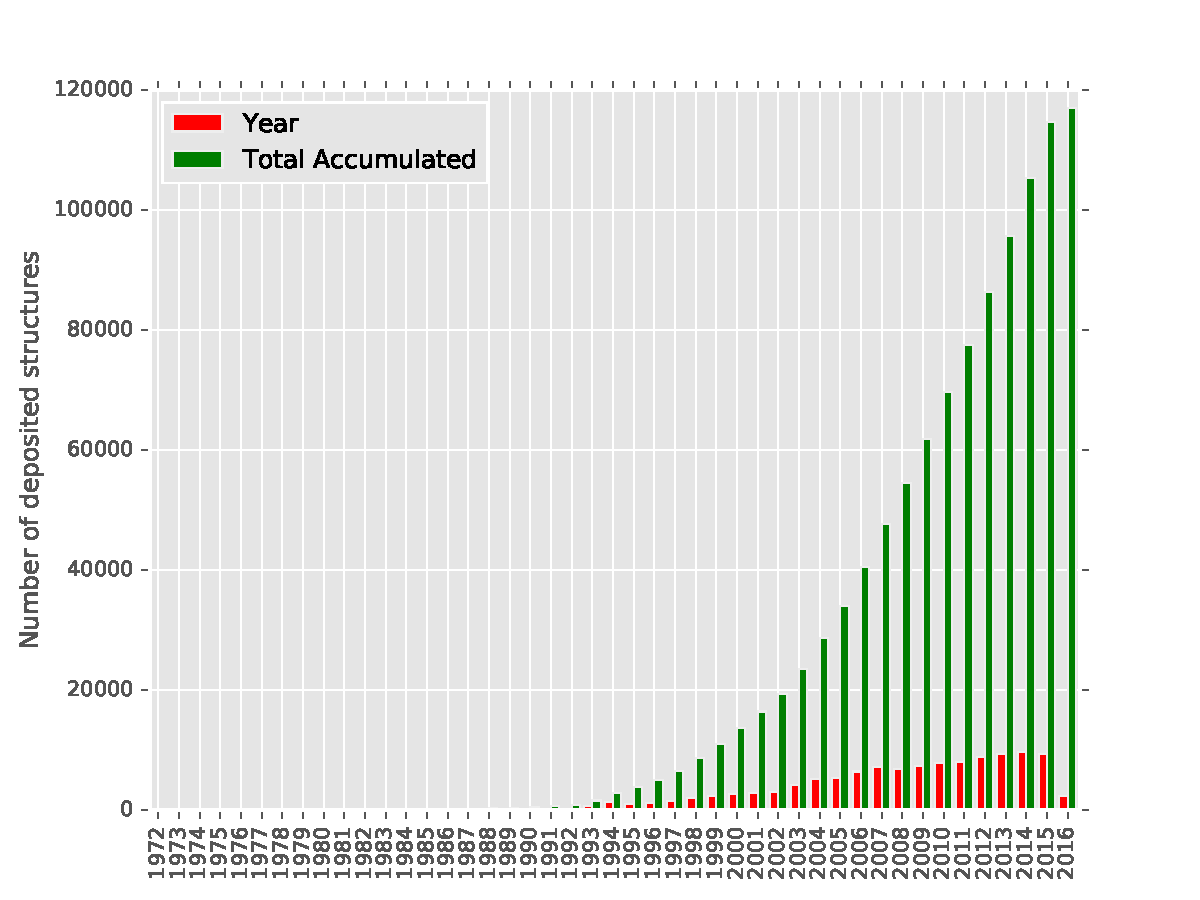
\includegraphics[width=1\linewidth]{../figures/pdbs_per_year.pdf}
	\caption{}
	\label{fig:structures_pdb}
	\end{subfigure}
	\begin{subfigure}[b]{0.55\textwidth}
	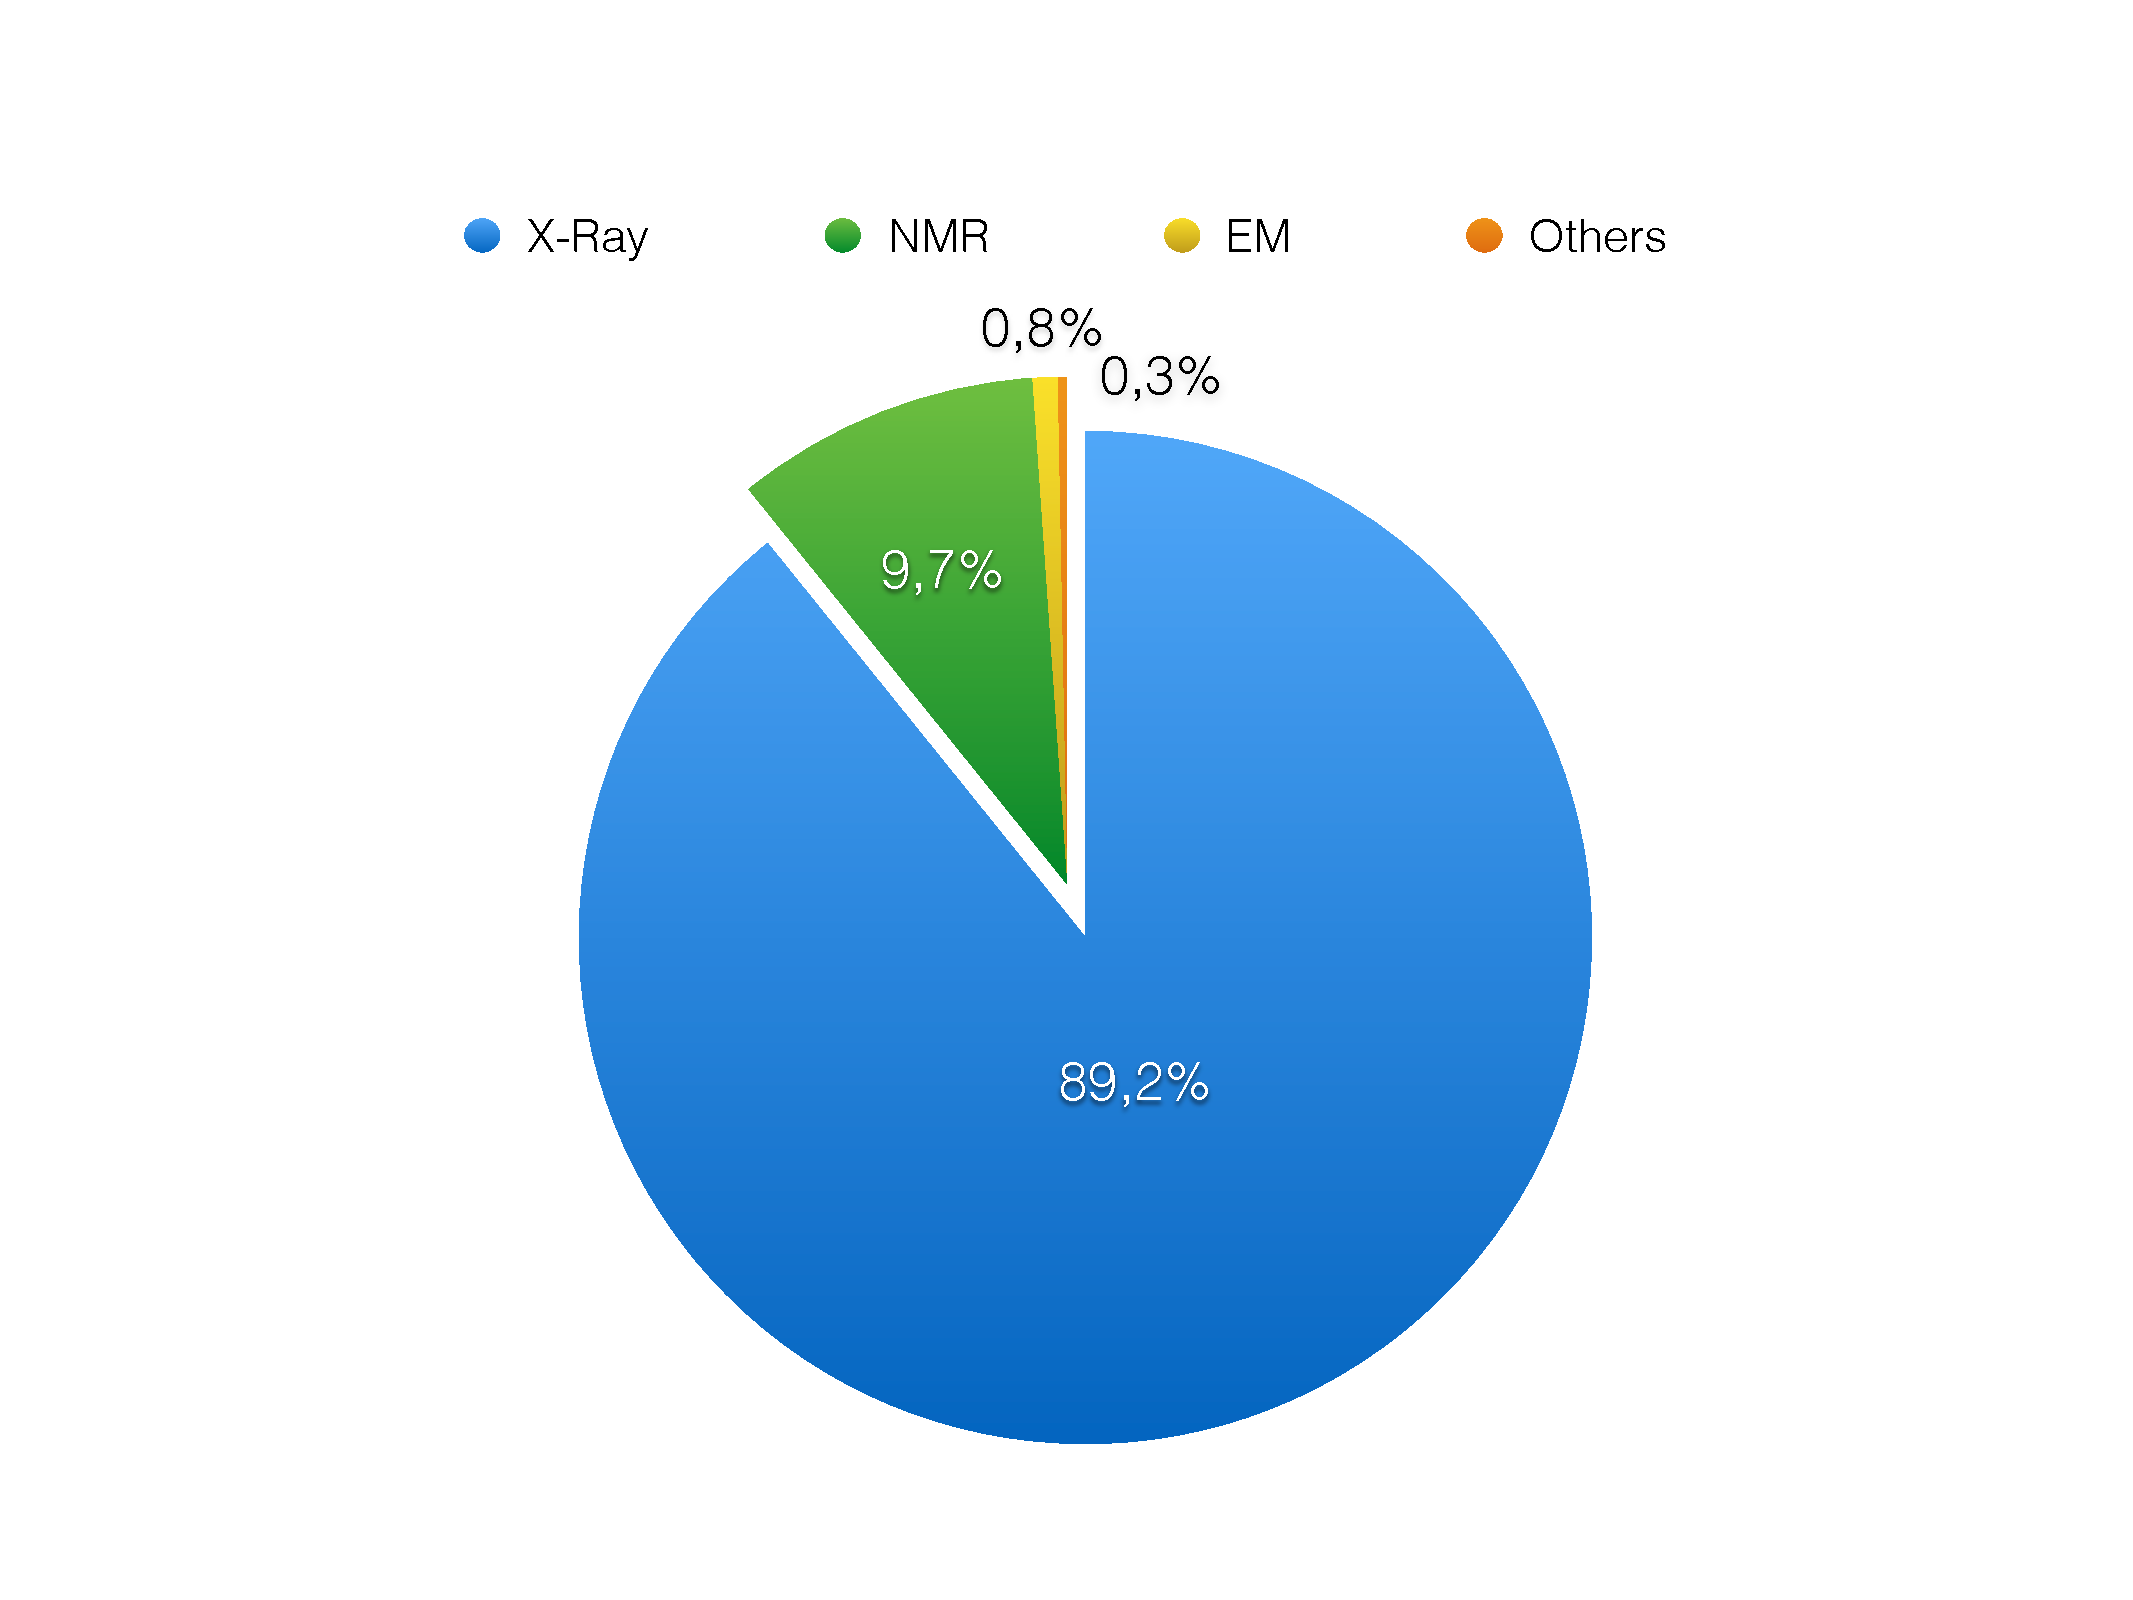
\includegraphics[width=1\linewidth]{../figures/pie_smethods.pdf}
	\caption{}
	\label{fig:smethods_pie}
	\end{subfigure}
   \caption{a) Growth of released structures per year. Data extracted from PDB. b) Pie chart with the percetange of structures determined by the different methods. Data extracted from PDB.}
   
	
	
\end{figure}


\pagebreak

\subsubsection{Protein Structure Prediction} \label{structure_predicion}


\par Despite of the advances in methods for protein structure determination, most of the known proteins lack of structure in the PDB. There are 550,740 annotated and curated protein sequences in UniProtKB (\url{http://www.uniprot.org}, April 2016).  However, only 4$\%$ of them (23,195 different protein sequences) have a link to a PDB structure. Therefore, there is a gap between the number of known protein sequences and the number of determined structures: the \textit{sequence-structure gap}. 
Computational methods for structure determination are helping to bridge this gap. The prediction of the 3D structure of a protein from its amino acid sequence has always been one of the most desirable goals in computational biology. It would save a lot of resources, and it would set a milestone in the structural biology field. Unfortunately, we are still far from being able to predict the structure of any protein from its primary sequence. Overall, four different approaches are commonly used. The first, and most extensively used, is the \textit{homology} or \textit{comparative} modeling, that uses similar experimentally determined structures to model the structure of the protein of interest \ref{Homology_modeling}. Second, \textit{fold recognition} and \textit{threading} methods are used to model protein structures with low similarity to known protein structures \cite{Jones1992, Bowie1991}. Third, \textit{de novo} or \textit{ab initio} methods make their predictions by combining the principles of physics that rule protein folding, with information derived from known structures but without relying in any type of similarity or evolutionary relationship to known folds \cite{Lee2009}. Finally, the \textit{integrative} or \textit{hybrid} methods combines different computational and/or experimental sources to perform the structure prediction \cite{Russel2012}.   
 
\subsubsection{Homology modeling} \label{Homology_modeling}

\begin{figure}[htb!]

  \centering
  	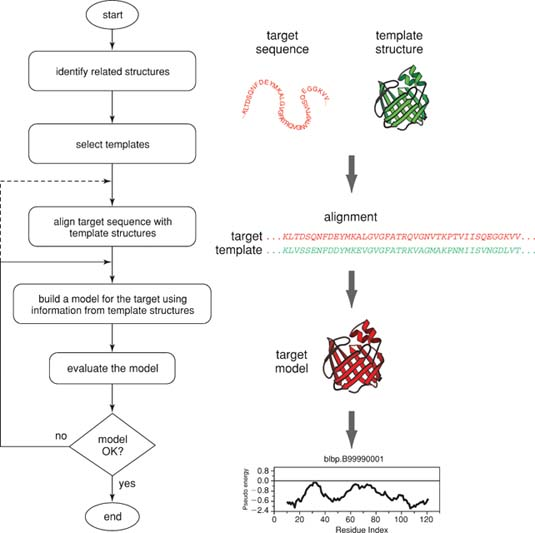
\includegraphics[scale=1]{../figures/workflow.jpg} % Figure was taking from...

	\caption{Workflow in comparative protein structure modeling.  The figure has been extracted from \cite{Eswar2007}}
	\label{fig:workflow_modeling}
\end{figure}
\par This type of protein structure prediction methods exploits the evolutionary relationship between the \textit{target} protein (i.e. protein being modeled) and the \textit{template(s)} with known experimental structure. They are based on the biological premise that evolutionary related sequences tend to have similar 3D structures. Figure \ref{fig:workflow_modeling} shows the regular steps in comparative protein structure modeling: 
\begin{enumerate}
\item \textbf{Identification of suitable template structures related to the target protein}. This step consist on a search for similar sequences with known 3D structure. This task is easy when a close homologue of the target protein has been solved. Initiatives such as the PSI\cite{Norvell2007} are helping in this issue increasing the number of modellable proteins. However, there are still many proteins with lack of homologous proteins in PDB. In these cases, alternative methods such as \textit{ab initio} modeling should be used.  

\item \textbf{Alignment between the target and the template(s) sequence(s)}. The sequence identity of the target-template alignment is the most frequently used measure for similarity. Consequently, the sequence identity is also a good predictor of the final 3D model quality. The overall accuracy of models calculated form alignments with sequence identity higher than 40$\%$ is usually good (i.e. RMSD\footnote{Root Mean Square Deviation is the measure of the average distance between the atoms of two superimposed proteins. Equation $RMSD=\sqrt[]{\frac{1}{N} \sum\limits_{i=1}^N \delta_i^2}$ where $\delta_i$ is the distance between the $N_i$ pair of equivalent atoms (usually the C$\alpha$).}  lower than 2.0\AA). In the 30$\%$-40$\%$ identity range, errors can be more severe and are often locate in loops and highly flexible regions. Below the 30$\%$ of sequence similarity, often referred to as \textit{twilight region}, serious errors occurs including the basic fold being mis-predicted \cite{Baker2001, twilight1996}.
Figure \ref{fig:homology_modeling} shows an empirical threshold for  homology modeling extracted from \cite{Sander1991}. The region below the curve covers those cases where the alignment does not carry enough information to model the 3D structure, while area above the threshold curve, include those cases where homology modeling is appropriate.  
\item \textbf{Modeling of the structurally conserved regions and prediction of the structurally variable regions.}. There are different algorithms to assign the spatial coordinates of the target protein using the template(s)-target alignment information. Highly conserved regions are generally well modeled, while those regions with insertions or gaps are more prone to include errors and sub-optimal atomic orientations. 

\item \textbf{Refinement of the initial model.} In this step the model is refined to idealize bond geometry and to remove errors that may have been introduced in the modeling step. The refinement process pursues the free energy minimization of the generated 3D protein model. Many different algorithms have been applied to perform the minimization step: molecular mechanics force fields \cite{PRO1410}, molecular dynamics \cite{Fiser2000}, Monte Carlo \cite{Kidera1995} and Genetic Algorithms\cite{McGarrah1993} are just several examples of the multiple approaches applied in this issue.
 
\item \textbf{Evaluation of the model(s).} Model evaluation seeks for the identification of the different errors that might have occurred during the modeling process. Multiple methods have been developed to assess the quality of a 3D model. In fact, 3D model assessment has a very such productive field for many years that it was included in the seventh edition of the CASP experiment \cite{PROT21669}. The general question of how accurate is a model can be reformulated in several specific questions: 



\begin{enumerate}[label=\roman*]
\item \textit{Is the selected fold correct?} The fold assessment consist of deciding whether a given protein model has the right fold. Residue-based combined accessible surface and distance-dependent scoring functions have shown the best performance in this task \cite{Melo2002}. 
\item \textit{How do we select the best model among the set of decoys or alternative solutions?} Several models can be generated by making changes in the template-target alignment, by selecting different template(s) structure(s) or by using different seeds in the refinement non-deterministic algorithms. Atom-based distance-depend scoring functions have proved to be useful for this particular task in some cases\cite{Samudrala1998}. However, there is not a gold standard for ranking the generated 3D models. Thus, the model selection eventually relies on the expertise of the person running the modeling. 
\item \textit{Which is the overall accuracy of the model? Which is the accuracy of the model in a particular region of the model?} These questions can be addressed by defining scores that correlates with the RMSD after superimposing a model and its native structure. Numerous scoring functions have been implemented to address this issue. Some of them, the \textit{physics-based scoring functions}, attempt  to  approximately  calculate the  atomic  interaction  energies  in  the  system.  These scoring functions usually encode a set of parameters that describes the energy of a system of particles. Examples of these scoring functions are AMBER\cite{CASE2005}, CHARMM\cite{Brooks1983} or MM-PDBSA\cite{Fogolari2003}. Differently the \textit{knowledge-based potentials} or \textit{potentials mean force} are scoring functions derived from an analysis of empirical information. Although the obtained scores are often considered approximations of the free energy, this physical interpretation is incorrect \cite{Thomas1996}. Nevertheless, since they frequently correlate with the actual free energy differences, they have been broadly used with significant success \cite{Shen2006, Zhou2002, Sippl1995}. 
\end{enumerate}
\end{enumerate}
\begin{figure}[h]

  \centering
  	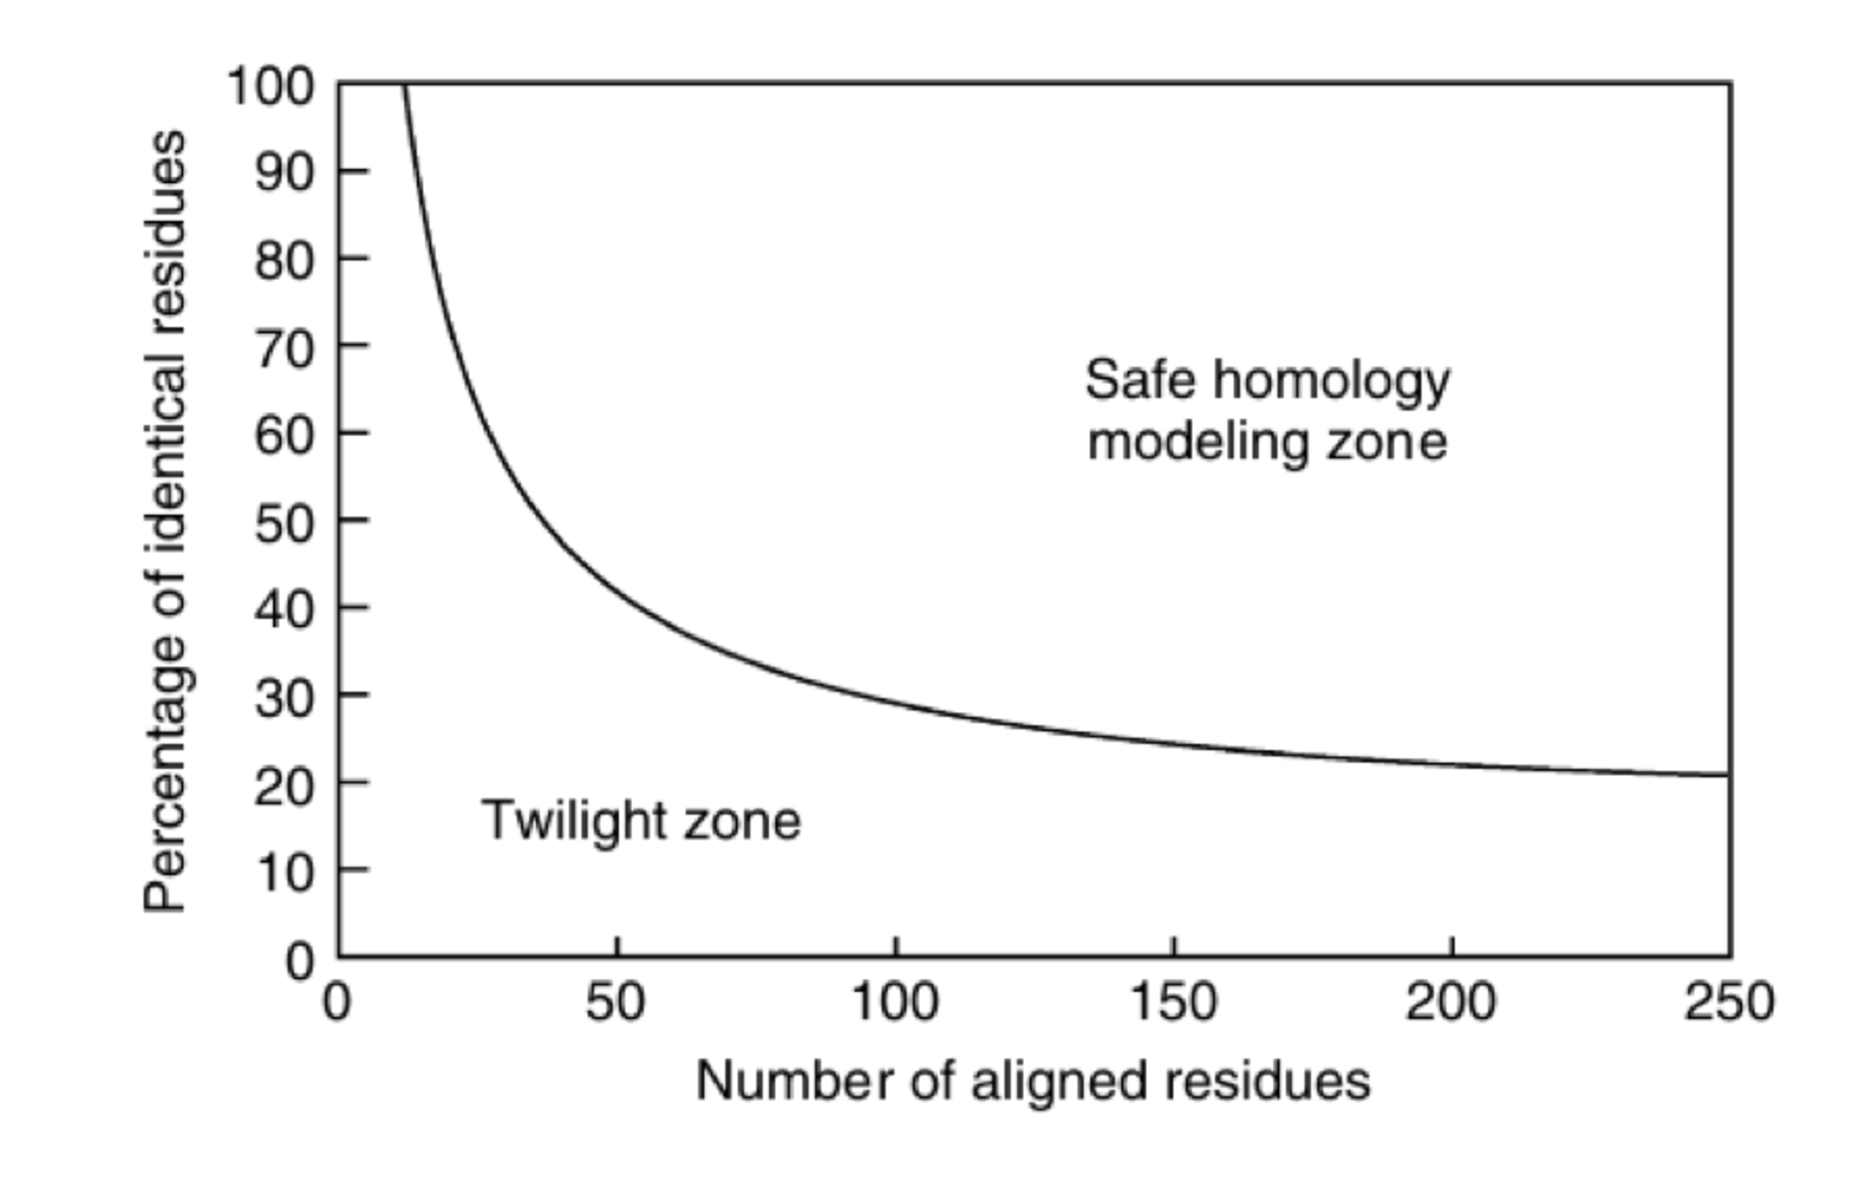
\includegraphics[scale=0.35]{../figures/homology_plot.pdf} % Figure was taking from...

	\caption{Homology threshold curve as a function of alignment length. Data extracted from \cite{Sander1991}}
	\label{fig:homology_modeling}
\end{figure}
\par The application of comparative modeling is limited by several aspects. The first one, is the availability of a suitable template. Despite of the efforts made to determine at least one structure per known fold \cite{Norvell2007}, divergences between the template and the target hampers the modeling of a correct 3D structure. In fact, models based on aligment below 30$\%$ have been shown to be unsatisfactory \ref{fig:homology_modeling}. The lack of template problem is even more noticeable in membrane proteins. The limited number available known membrane proteins structures makes its modeling an extremely difficult task. However, the high value of these proteins in diverse therapeutic areas \cite{Du2012, Kampen2011}, is fostering the development of specific membrane protein modeling methods \cite{Leman2015}. Another aspect that restricts the success of homology modeling is the innate flexibility of proteins. Highly flexible regions are more difficult to model and consequently are more prone to errors than more rigid parts of the structure. Despite of these limitations, homology modeling has been successfully applied to many proteins and its currently the main approach to computationally model the 3D structure of proteins\footnote{For a comprehensive review of homology modeling methods, applications and limitationsplease consider \cite{Marti-Renom2000, Malmstrom2010}}. 
\par There are many computational methods for predicting the 3D structure of proteins. Table \ref{table:table_software} shows some of the most famous ones alongside its websites and references. Each of these methods have their own strengths and weakness and none of them clearly outperforms the others for every case. In my case,  I have used Modeller because it is the one we are more familiar with. 
 
\renewcommand{\arraystretch}{1.2} %<- modify value to suit your needs

\begin{table}[h!]
 \centering
 \begin{adjustbox}{width=1\textwidth}
 \begin{tabular}{||c | c |c||} 
 \hline
 \tr\textbf{Modeling Tool}\br & \tr\textbf{Website}\br & \tr\textbf{Reference(s)}\br\\  
 \hline
 Modeller & \url{https://salilab.org/modeller/} & \cite{Eswar2007, Sali1993}  \\ 
 \hline
 SwissModel & \url{http://swissmodel.expasy.org} & \cite{Biasini2014} \\
 \hline
 HHPred & \url{http://toolkit.tuebingen.mpg.de/hhpred} & \cite{Soding2005}  \\
 \hline
 I-Tasser & \url{http://zhanglab.ccmb.med.umich.edu/I-TASSER/} & \cite{Yang2015a, Roy2010, Zhang2008}  \\
 \hline
 Rosetta & \url{http://robetta.bakerlab.org/} & \cite{Kim2004}   \\ 
 \hline
 RaptorX & \url{http://raptorx.uchicago.edu/} & \cite{Kallberg2014} \\
 \hline
 3DJIGSAW & \url{http://bmm.crick.ac.uk/~3djigsaw} & \cite{Bates2001} \\
 \hline 
  WhatIf & \url{http://swift.cmbi.ru.nl/whatif/} & \cite{Vriend1990} \\
   \hline
\end{tabular}
\end{adjustbox}
\label{table:table_software}
\caption{List of the public Protein Modeling Tools}
\end{table}




\subsection{Protein function}

\par The major question in the protein biology field has been to understand the protein sequence-structure-function relationship. It is known that structure of a protein determines its biological function. However, different \textit{regions} of the structure can perform semi-indepent functions from each other. These regions are referred to as \textbf{protein domains}. A domain is substructure produced by any part of polypedtide chain that can fold independently into a compact and stable structure \cite{Richardson1981, That1991, DomainDef}. Domains on average contain 80-250 residues \cite{Islam1995}. Estimates of the number of domains per protein say that more than 70\% of procaryotik proteins and 80\% of eukaryotic proteins include more than one domain \cite{Han2007, Chothia2003}. Among this multi-domain proteins, 95\% of them contains only two to five protein domains \cite{Han2007}.  Domains are not only the basic functional units of proteins, but also the evolutionary units of protein evolution. As proteins have evolved, domains have been modified and combined to build new proteins \cite{Vogel2004, Apic2001}. 
Such is the importance  of domains in protein evolution, that they have been included in current protein classification methods as one of the major classification parameters. Some of these domain classification methods such as SCOP \cite{Murzin1995} or CATH \cite{Orengo1997} are purely based on the structure, while others such as Pfam \cite{Bateman2002} or INTERPRO \cite{Hunter2009} include information about the function in their classification. 
\par Domains, and consequently proteins, perform its biological activity by interacting with other molecules. Proteins can interact with other proteins, constructing a protein-protein complex, with ions or with small-molecules. The substance that is bound to the \textit{target} protein is called the \textbf{ligand}, while the region of the protein where the ligand is binding is called ligand's \textit{binding site}\footnote{For simplicity, in this manuscript, unless otherwise indicated, the term ligand will only refer to small molecules ligands, while proteins ligands will be explicit named as protein-protein interactions}. The next section is focused on protein-compound interaction and it presents the basis for all the work developed during the thesis. 



\subsection{Protein-Ligand Interactions} \label{ligand_intect}


\par The roles played by the protein ligands are diverse. Catalysis of enzyme substrates, regulation of the protein activity, cellular communication or defense from external attackers are just few some examples of the multiple functions that small-molecule ligands perform in living organisms. All these functions are performed by small-molecules that selectively bind their \textit{target} proteins. However, given the vast amount of proteins and small-molecule ligands in the cytoplasm, how do the small-molecule ligands select their protein targets? There has been several protein-ligand binding theories. In the \textit{Lock and key Theory} \cite{Cramer1994}, Emil Fischer proposed a system where the binding sites of enzymes are rigid and pre-adjusted geometrically to the natural substrate \ref{fig:lock_and_key_model}. This theory became widely accepted for years. Nevertheless, during subsequent years, evidence started to accumulate suggesting that the binding sites of proteins do not match perfectly their ligands, but rather the binding process triggers some conformational changes in the enzyme. Therefore the obsolete Lock and key model was replaced by the \textit{Induced fit theory} \cite{Koshland1959}. The induced fit theory proposes that initially enzymes do not perfectly match their substrate geometrically. However, the binding-process triggers a set of conformational changes in the protein binding site that improves the match \ref{fig:induced_fit_model}. More recently, another theory called the \textit{Monod-Wyman-Changeux model or  MWC model } came up\cite{Monod1965}. This theory contends that proteins are able to shift spontaneously between multiple conformations called \textit{substates}\cite{Kitao1998, Petsko1984}. This model could also explain \textit{allostery}, a phenomenon in which the binding of the molecule to the catalytic site is affected the binding of other ligand to a different site. This theory has undergone some changes and the current accepted theory posits that ligands bind preferentially to one of the conformation sampled spontaneously by the protein, and therefore stabilizes it. It means that, by changing the protein's energy landscape, ligands change a less favorable conformation into the most favorable one. This model does not necessarily refute the induce fit theory since in many cases, the restrains applied by the ligand on the binding site is expected to induce some conformational changes that will further stabilize the interaction \cite{Foote1994, James2003}. 

\begin{figure}[!tbp]
  
  \centering
    \begin{subfigure}[b]{0.75\textwidth}
	
\includegraphics[width=1\linewidth]{../figures/lock_key_model.jpg}
	\caption{Fischer's \textit{lock and key model}. The protein is represented in green and the ligand in red. The ligand's binding site of the protein matches the ligand perfecltly.}
	\label{fig:lock_and_key_model}
	\vspace*{4mm}
	\end{subfigure}
	\begin{subfigure}[b]{0.75\textwidth}
	
\includegraphics[width=1\linewidth]{../figures/induce_fit_model.jpg}
	\caption{Koshland's \textit{induced fit model}. The protein is represented in green and the ligand in red. The overall shape of the ligand matches the binding site. The ligand bindings causes some conformational changes that improves the interaction.}
	\label{fig:induced_fit_model}
	\vspace*{4mm}
	\end{subfigure}
	\begin{subfigure}[b]{0.75\textwidth}
	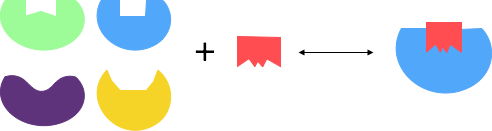
\includegraphics[width=1\linewidth]{../figures/mwc_model.jpg}
	\caption{\textit{MWC model's} representation. The protein changes its conformation constantly (one color per conformation), with at least one these conformation matching the ligand. Its binding triggers some conformational changes that improves the protein's energy landscape.}
	\label{fig:mwc_model}
	\vspace*{4mm}
	\end{subfigure}
   \caption{Schematic representation of three popular protein-ligand binding theories.}

\end{figure}
\subsubsection{Protein-ligand binding energetics}\label{binding_energetics}

\par The high variety of functions that ligands perform by binding to proteins its also reflected in the diversity in its binding affinity. Binding energies usually range from -2.5kcal/mol to -22kcal/mol \cite{Dunn2001}. The binding strength displayed by proteins matches the biological goal of the binding. For instance, ligands involved in protein communication tend to bind weakly to enable a quick state switch. Cofactors binding to enzymes, on the other hand,  tend to bind strongly to their targets.  The negative sign of the values reflects that is a favorable binding that releases energy: \textit{the binding free energy}.  This energy can be measured experimentally, thorough the equilibrium constant of the binding, or it can be calculated computationally. Equations \ref{equation: Gibbs free energy} and \ref{equation: Kbind} shows, under thermodynamic equilibrium conditions, the relationship between the Gibbs free energy or binding affinity and the equilibrium constant of the binding. $R$ is the ideal gas constant [ref], $T$ is the temperature , $[C]$ the complex concentration and $[P]$ and $[L]$ the protein and ligand concentration respectively. 
\begin{equation}\label{equation: Gibbs free energy}
\bigtriangleup G=-RTlnK_{bind} 
\end{equation}
\begin{equation}\label{equation: Kbind}
Kbind = \frac{[C]}{[P]*[L]}
\end{equation}
\par These equations show that the binding free energy can be measured experimentally. However, in many cases the experimental measurement are unfeasible or very difficult due to technical problems. Additionally, the expenses associated with these experiments often restricts its broader application. In such cases, computational methods to calculate the free binding energy are needed. The calculation of binding free energy have acquired a remarkable importance in the drug discovery field where the calculation of ligand-target affinity is crucial for the pre-clinical phase \ref{drug_discovery}. Unfortunately, its calculation its a extremely challenging task. The main points that should be addressed to accurately calculate the binding free energy are: 
\begin{enumerate}
\item \textbf{The free energy of binding \ref{equation: Gibbs free energy} is the difference of two large energies}. The energy of the complex ($E_{pl}$) and the energy of the unbound partners ($E_{p} + E_{l}$) \ref{equation:energy_complex}: 
\begin{equation}\label{equation:energy_complex}
\bigtriangleup G_bind=E_pl - (E_{p} + E_{l}) 
\end{equation}
\item \textbf{There are two opposite and complex energies driving the process}. The binding enthalpy ($\bigtriangleup H_{bind}$) and the loss of entropy of both the ligand and the protein ($\bigtriangleup S_{bind}$): 
\begin{equation}\label{equation:energy_enthalpy_entropy}
\bigtriangleup G_bind= \bigtriangleup H_{bind} -  T\bigtriangleup S_{bind} 
\end{equation}

\item \textbf{Non explicit representation of the energetic interactions of the system}. Small-molecule binding events on a protein cavity implies the displacement of solvent molecules (usually water molecules). The energy generated by the this exclusion of water molecules is the main driving force in ligand-protein binding \cite{Michel2009a}. Unfortunately, explicit representation and simulation of all the forces involved this event is computationally unfeasible. A popular approach to model is to use implicit solvent theories \cite{Ravindranathan2011, Michel2006, Liu2009}, where the water molecules are represented as a continuous medium instead of individual explicit molecules. The implicit solvation model is justified in liquids, where the potential of mean force are applied to approximate the behavior of many highly dynamic solvent molecules. However, there could be other medias with specific solvation or dielectric properties that are continuous, but not necessarily uniform, since their properties can be described by different analytic functions \cite{Lu2007}. Within the most famous implicit models we can find those based on those based on Boltzmann theory (PB) \cite{Sharp1990} and those based on Generalized-Born (GB) approximation \cite{Bashford2000}. 
\par Hydrogen bonds and salt bridges between the ligand and the protein can also be a source of free energy gain upon ligand binding. This energy gain comes from the displacement of water molecules bound to the protein. The net gain of energy upon hydrogen bond is around 1-2 kcal/mol. Some scoring functions treat all hydrogen bonds equally, while others, distinguish between neutral and charged ones. Other energies that could be modeled and that contribute to the binding affinity calculations are those generated by interactions with metal ions \cite{Friesner2004}. However, because there can be a covalent component in this type of interactions, its overall binding energy contribution is difficult to model. Finally, nonspecific van der Waals and hydrophobic interactions are also included in some methods as additional energy contributors to the overall free energy of binding \cite{Steffen2010}. 
\end{enumerate}

\par One of the main applications of binding free energy calculation is predicting whether a ligand is binding a particular protein target. In other words, given the predicted binding free energy determine whether a specific compound targets a specific protein binding site. In the next section we will explore further these and other approaches aiming at protein-compound interaction prediction.  




\subsubsection{Protein-ligand prediction}\label{prediction ligand-target}

\par  \footnote{In chapter [REF] we present nAnnolyze, a method for protein-ligand interaction prediction. In the introduction of the presented manuscript, there is a discussion of the current state-of-the-art methods in protein-ligand interaction prediction. Therefore, this section is focused in explaining the classification, underlying basics and (dis)advantages of the different approaches.} The importance of ligand-protein interaction prediction is reflected by the large number of available methods that use multiple different approaches \cite{Csermely2013, prathipati2015}. We can distinguish between \textit{free structure} methods (i.e. methods that do not rely on the protein structure to perform its predictions) and \textit{structure-based} methods.    
\par Free structure methods do not require the protein structure to perform their predictions. They usually use prior knowledge on protein compound interactions, to further extend the interactions to new and unseen compounds. The development of these methods can be split in two phases. The first step consist on the creation of a predictive model that uses a collection(s) of protein-compound interactions to learn hidden relationships between compound and their protein targets.  In the second step, these predictive models are used to extrapolate this knowledge to new and unseen compounds (or targets). The extrapolation relies on different types of compound or protein similarity. Knowledge-based free structure methods have been assisted by the advent of new and powerful \textit{high-thorughpout screening methods} (HTS) that allowed the creation of large computational compound-protein databases such as ChEMBL \cite{Bento2014},Therapeutic Target Database (TTD) \cite{Zhu2012a}, Binding MOAD \cite{Hu2005}, BindingDB \cite{Liu2007}, PubChem \cite{Kim2016, Wang2014} or ZINC \cite{Irwin2012}. The recent growth of these collections is accordingly improving these method's accuracy and coverage. Moreover, since they do not rely on protein structure they can be theoretically applied to any protein or any compound. Nevertheless, free structure methods do not provide detailed information about the ligand-protein relationship. Information such as binding localization, type of interaction (i.e. allosteric, on-target or off-target) or predicted free energy of binding;  that is absolutely essential in the drug discovery process. Consequently ,free structure methods are mostly employed in very early stages of the drug discovery pipeline. 

\par Structure based target prediction methods use the protein structure to determine whether a small-molecule interact with a protein target. Docking methods have traditionally dominated the structure-based target prediction field. Virtual docking consist on predicting the preferred orientation of one molecule (the ligand) to a second (the protein) one. The process of finding the best orientation of molecule (i.e. its \textit{pose}) to its protein target is not simple, since several entropic, enthalpic and environmental factors have an impact on the interactions between them \ref{binding_energetics}. The underlying idea of this approach is to generate a comprehensive set of ligand-protein conformations, and then to rank them according to a specific scoring function \cite{Alonso2006}. The importance of virtual docking methods is not only reflected by the large number of published methods  (AutoDock \cite{Morris2009, Trott2010}, DOCK \cite{Ewing1997}, FLEXX \cite{Rarey1996}, GOLD \cite{Jones1997} and GLIDE \cite{Friesner2004} among others), but also by their success in drug discovery applications \cite{Schames2004, Enyedy2001, Vangrevelinghe2003}\footnote{For a comprehensive review of virtual docking methods an applications please consider \cite{Kitchen2004}}. However, virtual docking methods also have some limitations. The most apparent one is that they do rely on protein structure. As explained above \ref{structure_predicion} the coverage of the human structural proteome is below 40$\%$. Thus, some of the most interesting targets in drug discovery lack of experimentally determined 3D structure. In addition to these structurally inherent  problems and despite of some massive applications \cite{Reardon2013},  virtual docking methods are still computationally very expensive. Additionally, they need the prior knowledge of the binding localization in the protein surface which many times is unknown before the screening. To overcome the computational limitations, new structure-based methods use the so-called \textit{comparative docking} approaches that solely rely on structural comparisons, both of compounds and protein targets, to infer new interactions [REFS]. Chapter [REF nAnnolyze] presents nAnnolyze, a method to predict ligand-target interactions using a comparative docking approach. In that chapter it is further discussed the applications and limitations of these type of approaches. 


\section{Drug discovery}\label{drug_discovery}

\par Drug discovery is the process by which potential new potential medications are discovered. It involves a wide range of scientific disciplines, including biology, chemistry, pharmacology and recently also the computational branches of these fields. Historically, drugs were discovered through the identification of the active ingredient from traditional remedies or by serendipitous discovery. Later, the development of synthetic methods allowed the generation of purely synthetic structures that were not found in nature and that were investigated as potential therapeutic agents. More recently, the advent of new genomics, proteomics and high throughput screening (HTS) techniques, resulted in the identification of large number of novel targets for future drug research. In addition to this \textit{technological revolution}, the advances in bioinformatics and system biology field has prompted the change in drug discovery paradigm towards a more target-centric approach. This \textit{modern drug discovery paradigm} usually implies the screening of thousands of molecules in order to identify those that have the desirable therapeutic effect in the previously validated protein target \cite{Drews2000, Patrick2001}. Figure \ref{fig:drug_discovery_pipeline} shows the current drug discovery pipeline alongside the estimated cost and time of each of the phases.  Most modern drug discovery programs begin with the identification of a bio-molecular target which pharmacological intervention is theoretically beneficial for the treating disease. A target is a broad term which can be applied to a range of biological entities which include proteins, DNA and RNA. The target needs to be accessible to the putative drug molecule(s), this property is called as \textit{target druggability}. Wrong selection of the target (i.e. weak association between the target and the treating disease) implies lack of the expected efficacy, which is the most important cause of project failure in clinical trials\cite{Hutchinson2011, Lindsay2003}. During the \textit{Target-to-hit} stage, the target is screened against a set of candidate molecules seeking for the identification of those which able to perform the desired therapeutic activity. Alternatively, in some cases the first step of the discovery process is based on a \textit{Phenotypic screening} of a collection of molecules. This screening pursues the identification of those molecules that perform a predefined function in a biological model. In any case, prior knowledge of the bio-molecular target of the therapeutic activity is generally associated with better outcomes in clinical trials \cite{Hughes2011}. However, there are various drugs in the market with unknown \textit{mechanism of action} (i.e. the drug target is still unknown) \cite{Imming2006}, most of them coming from the traditional drug discovery paradigm.  After this hit(s){\footnote{ A hit compound could have several definitions. Here we use the one from \cite{Hughes2011}  where they defined a hit as being a compound which  \textit{has  the  desired  activity  in  a  compound  screen  and whose  activity  is  confirmed  upon  retesting}}   identification, in the \textit{hit-to-lead} stage,  molecular hits are evaluated and undergo limited optimization to identify promising lead compounds for further stages. The optimization to convert a hit to a lead molecule, implies several properties. Properties such as the potency, the selectivity or the pharmacokinetics (PK) properties [hablar en computational methods, SAR]. These lead compounds undergo more extensive optimization in a subsequent step of drug discovery called lead optimization (LO). The main goal of this stage is to maintain favorable properties in lead compound(s) while improving on deficiencies in the lead structure(s). Finally, the selected lead(s) enters into the preclinical stage where the main goals are determining the safe dose for \textit{First-in-man study} and the first assessing the product's safety profile. Estimates say that, on average, of every 5,000 to 10,000 compounds that begins the pre-clinical stage, only one becomes an approved drug \cite{Klees1997}. 

\begin{figure}[!tbp]
  
  \centering
    
	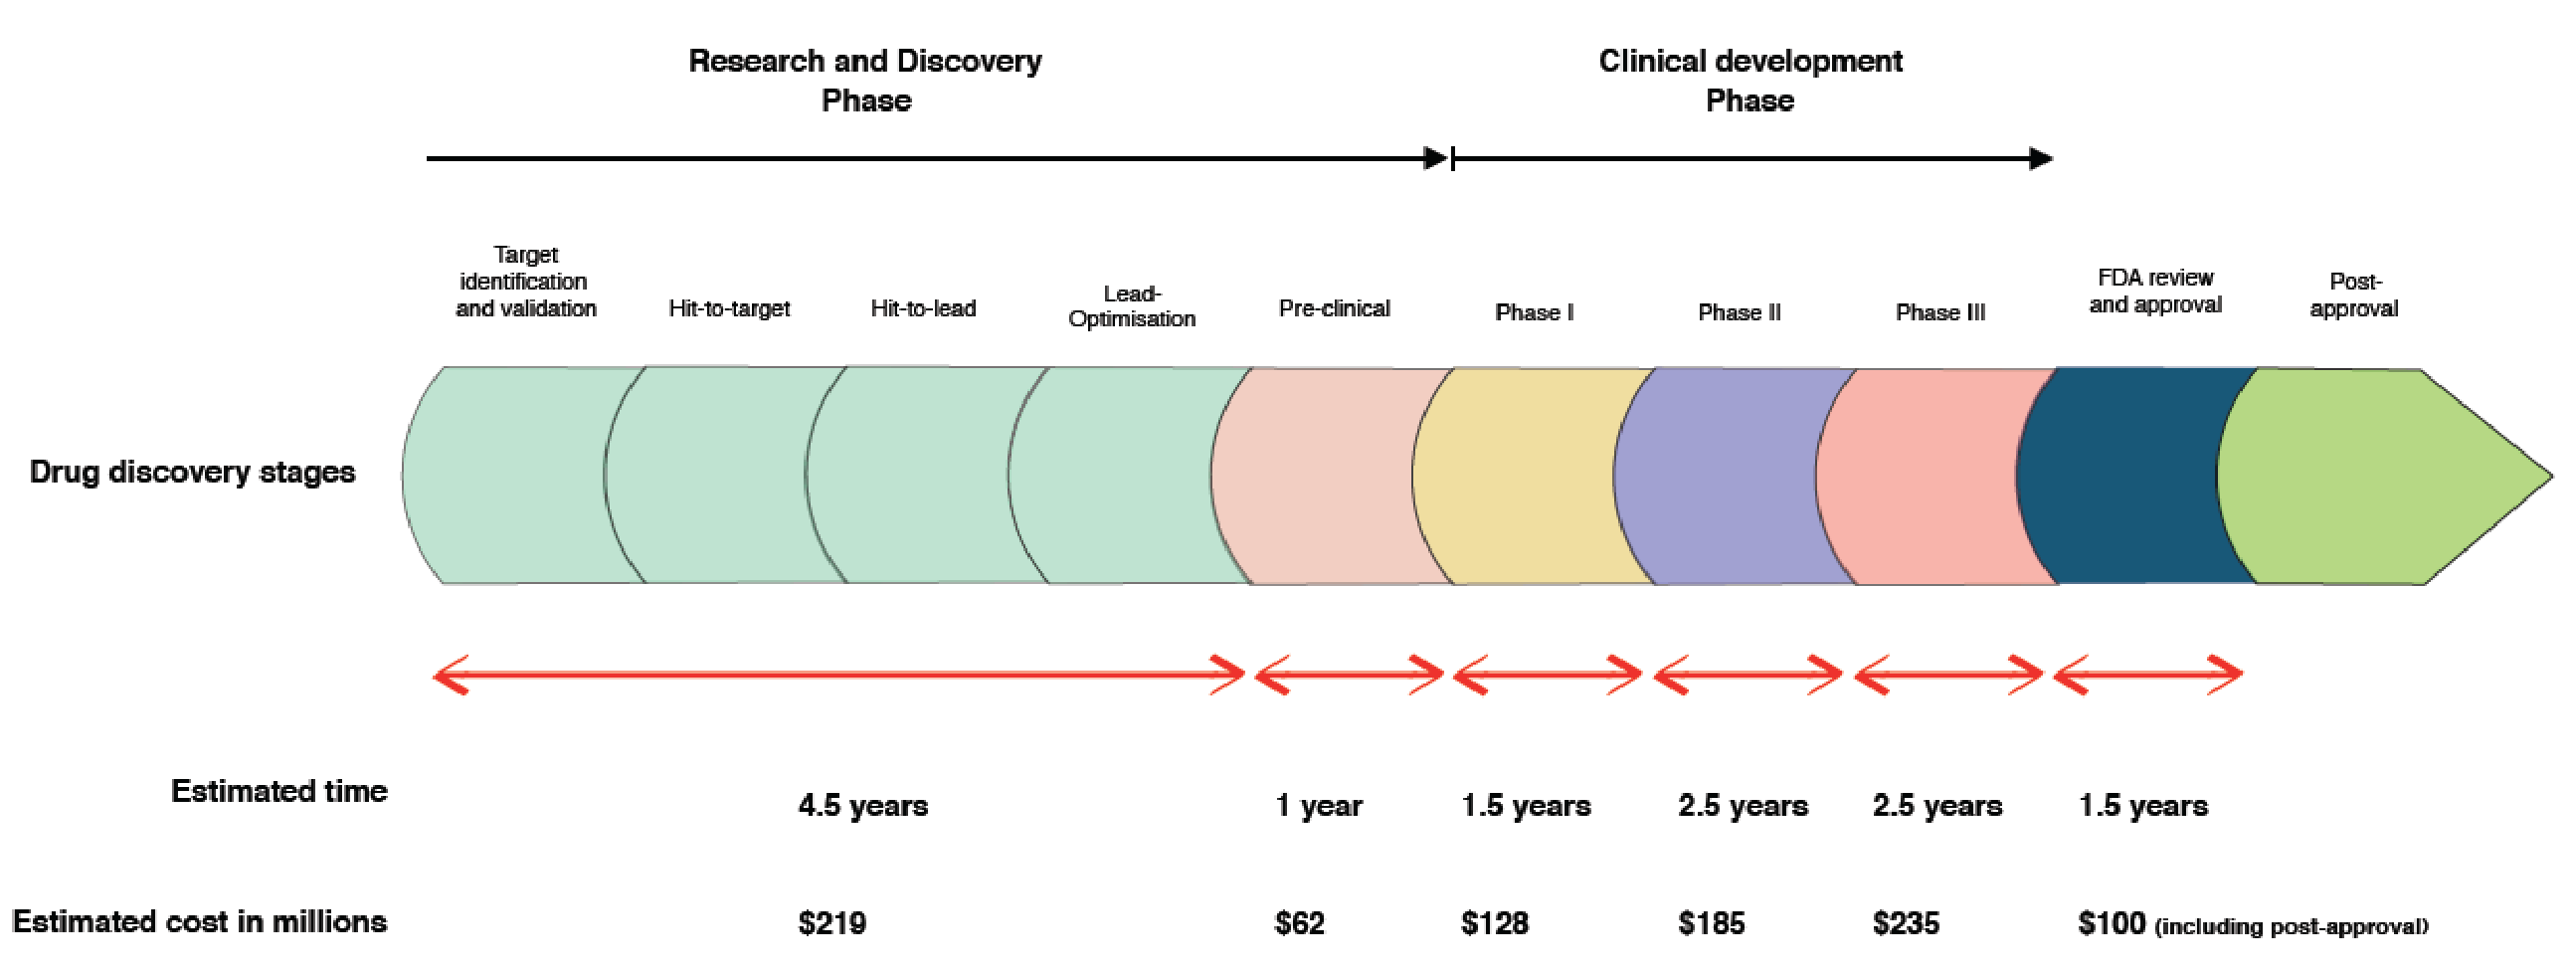
\includegraphics[width=1.0\linewidth]{../figures/drug_discovery_pipeline.pdf}
	\caption{Drug discovery and development pipeline. For each stage the average cost and time are included. Post-approval times not included in the time-line. Data extracted from \cite{Paul2010}.}
	\label{fig:drug_discovery_pipeline}
	%\vspace*{4mm}
\end{figure}


\par  According to the The Tufts Center for the Study of Drug Development (\url{http://csdd.tufts.edu}), the development and marketing approval for a New Molecular Entity (NME) takes more than 13 years and around  $\$$2.6 billion \ref{fig:drug_discovery_pipeline}. In fact, the cost of developing a new drug has dramatically increased since the 1970s \ref{fig:drug_discovery_evolution}. Currently,  the cost of developing a NME is more than two times the 1990s one, and more than ten times of the cost in the 1970s.   
This raise in the drug development cost has lead to a dramatic shrinkage of the efficiency, measured in terms of the number of new approved drugs per billion US dollars of research and discovery (R$\&$D) spending \cite{Scannell2012}. Both research and development phases have significantly raised their expenses \ref{fig:drug_discovery_evolution}. Factors that have contributed to the raise of clinical costs include increased clinical trial complexity, larger clinical trial size, greater assessment of safety and toxicity drug profiles or evaluation on equivalent drugs to accommodate payer demands for comparative effectiveness data \cite{Scannell2012}. Similarly, factors such as the complexity of the target disease, expenses associated with the application of high-throughput technologies or the increased complexity of mechanism of action are boosting the prizes of pre-clinical stages. However, pre-clinical associated expenses could be narrowed down with a rational use of the state-of-the-art technologies. In this matter, computational methods are emerging as a tool to speed-up by allowing the management of the massive amount of data generated during the discovery stages. The next section presents different computational methods currently applied during the drug discovery pipeline.  
\begin{figure}[!tbp]
\centering
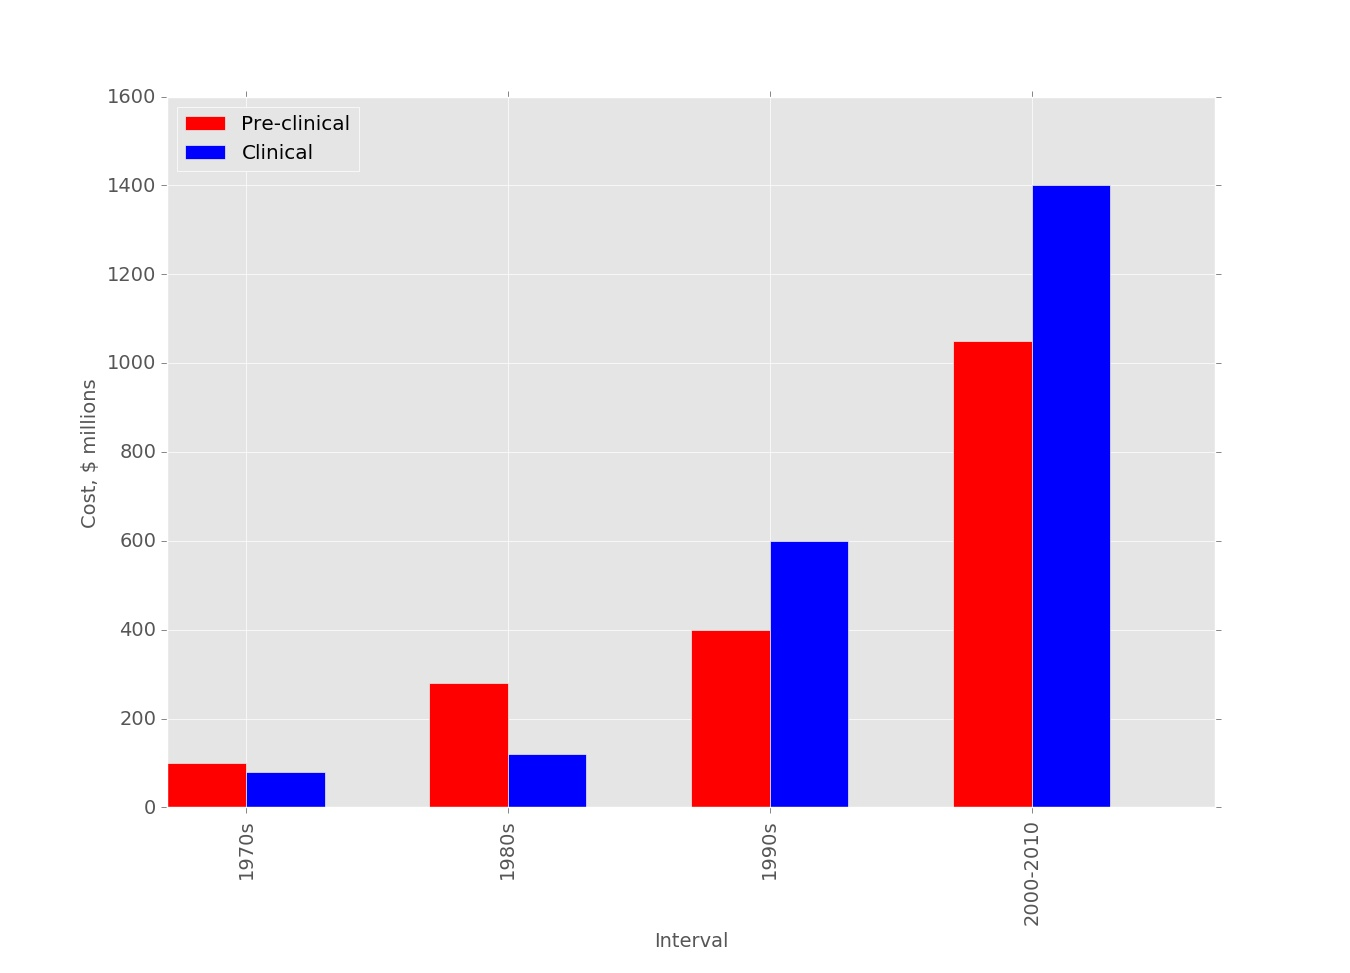
\includegraphics[width=0.9\linewidth]{../figures/drug_discovery_evolution.jpg}
	\caption{Cost of developing a new drug. Blue bars indicate expenses in clinical phases while red represents expenses in pre-clinical stages. Costs are shown in $\$$ millions. Data extracted form: Tufts Center for the Study of Drug Development (\url{http://csdd.tufts.edu/news/complete_story/pr_tufts_csdd_2014_cost_study}).}
\label{fig:drug_discovery_evolution}
	
	\vspace*{4mm}
\end{figure}
  

\subsection{Computational drug discovery}\label{computational drug discovery}

\par Over the last thirthy years, computer-aided drug discovery (CADD) methods, have played a key role in the development of therapeutic drugs \cite{Sliwoski2014}. The modern drug discovery pipeline includes multiple CADD approaches that assist during the drug discovery process:

\begin{enumerate}

\item \textbf{Target identification and validation methods.} Many different computational approaches are used to identify and validate new targets. The \textit{the genomics revolution} caused by New-Generation Sequencing methods (NGS) have boosted the development of methods that primary rely on the genetic association between targets and the treating diseases. Sometimes, these data is combined with additional information that allows a better evaluation of the target viability. This complementary information include structural data,  such as experimental structure availability or druggability assessment; system-biology information such as protein-protein interactions, protein pathway analysis or sub-celullar target localization \cite{Yang2009}. Recently, the inclusion of pharmacological data by \textit{drug reporpousing or repositioning} methods is becoming very popular \cite{predict, Zhang2011, YutakaFukuoka2013}. These methods uses information of whether the protein is targeted by any FDA approved drug. This information is used then to prioritize those targets with annotated FDA approved drug(s). Such drug(s) are subsequently applied to the treating disease to validate the target testing hypothesis. Computational methods for target identification and validation have applied in great variety of diseases: from infectious diseases such as Tuberculosis \cite{Raman2008} or Malaria \cite{Phaiphinit2016}, cancer \cite{Jeon2014} to neurogeneretive diseases \cite{Augustin2012}. 

\item \textbf{Ligand-target prediction}. Once the target has been validated, CADD methods can help in the search of potential target hits. This is one of fields where CADD methods have been more successful either by making the predictions from scratch or in combination with phenotypic screenings \cite{Martinez-Jimenez2013}. Section \ref{prediction ligand-target} specifies the different methods and its current applications.   

\item \textbf{Quantitative structure-activity relationship (QSAR)}\label{qsar}. QSAR is an approach designed to find relationships between chemical structure and the biological activity of small molecules. QSAR methods are based on the assumption that variations in the biological  activity  of  a  series  of  chemicals  targeting a particular protein are correlated  with variations in their structural, physical, and chemical properties \cite{Perkins2003}. QSAR methods have become an essential tool in the pharmaceutical industry where they a major role in the hit-to-lead and lead optimization stages. Traditionally, these methods have been used to improve compounds bioactivity. Recently, the applications have been extended to the improvement of ADMET (adsorption, distribution, metabolism, elimination, toxicity) properties \cite{Penzotti2004, Obrezanova2007} and the oral bio-availability \cite{Yoshida2000}. QSAR  methods have undergone rapid changes over the last years. The first 2D-QSAR models were based on descriptors derived from a two-dimensional graph representation of a molecule. These descriptors tried to characterize the most important molecular properties for the molecular interaction. However 2D-QSAR has important limitations for designing new molecules due to the lack of consideration of the 3D structure. 3D-QSAR emerged as a extension to the classical 2D-QSAR approach, which exploits the three-dimensional properties of the ligands to predict their biological activities \cite{Verma2010}. The first QSAR model that integrated the 3D geometry to perform the predictions was the Comparative Molecular Field Analysis (CoMFA) \cite{Cramer1988}. In CoMFA, steric and electrostatic features of protein target are mapped onto a surface grid, which envelops a set of compounds superimposed in their active conformation. This grid acts as a surrogate of the binding site of the protein receptor and its frequently referred to as \textit{pharmacophore}. However, this approach has an important limitation: a ligand molecule can only be represented by a single entity. Therefore, if a ligand binds with different conformations, only one of them can be represented in a 3D-QSAR model \cite{Verma2010}. This limitation was overcome by 4D-QSAR methods, which include conformational flexibility and the freedom of alignment by ensemble averaging in the conventional three dimensional descriptors found in 3D-QSAR methods \cite{Hopfinger1997}. 4D-QSAR models have been succesfully applied to simulate binding to cytochrome P450 3A4 \cite{Ekins2000}, HIV-1 protease \cite{Iyer2007} or to the p38-mitogen-activated protein kinase (p38-MAPK) \cite{Romeiro2010} among others \cite{Andrade2010}. More recently, a 5D-QSAR model have been proposed \cite{Vedani2002}. This models includes a degree of freedom, the fifth dimension, that allows for a multiple representation of the atomic topology of the receptor surrogate (i.e. representation of different induced-fit models of the receptor). Finally, in the 6D-QSAR methods, a greater representation of the different solvation scenarios is included \cite{Vedani2005}. This allow for an even more realistic simulation of the binding process which ultimately is reflected in the development of better predictive models.   
\item \textbf{Prediction and optimization of the ADMET properties}. Most of the drug discovery initiatives include a computational optimization of the compound's PK properties. As previously mentioned, QSAR methods have been extensively applied to predict the PK properties of compounds \ref{qsar}. However, there are other \textit{in-silico} approaches that play a substantial role in the ADMET prediction field.   One of the tools that have significantly contributed to the field is the \textit{Lipinski's rule-of-five} , which aims to predict the odds of a compound to become a drug: \textit{the compound drug-likeness} \cite{Lipinski2004}. The Lipinski's rule-of-five is a rule of thumb created by Christopher A. Lipinski based on the observation of chemical properties of drugs with favorable PK profile. It uses five arbitrary rules based of such number of chemical features to determine whether a compounds is likely to become a drug. If the compound fulfill (at least) four rules then it is considered as a drug-like candidate. However, assessment of compounds drug-likeness in absolute terms does not reflect adequately the whole range of compound qualities. To address this issue, a computational method that quantitatively measures the drug-likeness of a compound has been recently pubilshed \cite{Bickerton2012}. Optimization in the ADMET properties of a compound is generally performed during the hit-to-lead and lead-optimization stages, concurrently with the optimization of the compound's bio-activity. This multi-objective optimization process is brilliantly accomplished in the computational model developed by Besnard and colleagues \cite{Besnard2012b}.\end{enumerate}


\section{Drug discovery in Tuberculosis}}

\par About one-third of the world's population is infected with \textit{Mycobacterium tuberculosis} (MTB), the causative agent of tuberculosis (TB) \cite{Lewandowski2015}. Approximately 95$\%$ of infected individuals have latent MTB infections, which remain dormant until activated by specific environmental and host response events. Approximately 10$\%$ of latent infections eventually progress activating the disease. However, people with compromised immune systems, such as people with HIV, malnutrition or diabetes, or people who use tobacco, have a much higher risk of falling ill. Once the disease has been activated, when left untreated, kills more than half of the infected patients \cite{Connell2011}. Despite of TB is considered as a treatable and curable disease, it remains as a top infectious disease killer worldwide. TB is usually treated with a standard 6 month course of combination of 4 antimicrobial drugs. Globally, the treatment success rate for people newly diagnosed with TB was 86$\%$ in 2013 \cite{Lewandowski2015}. Unfortunately, there is a increasing clinical occurrence of Multidrug-resistant tuberculosis (MDR-TB), which is a form of TB caused by bacteria that do not respond to first-line anti-TB drugs. In some cases, more severe drug resistance can develop such as the Extensively drug-resistant TB (XDR-TB), which is a form of MDR-tb tuberculosis that do no respond to any standard treatment, including the most effective second-line anti-TB drugs \cite{Berry2009}. About 480,000 people developed MDR-TB in the world in 2014 while it is estimated that about 9.7$\%$ of MDR-TB cases had XDR-TB \cite{Lewandowski2015}.

\par Infectious diseases in general, and TB in particular, are suffering from the lack of new innovative therapies \cite{Trouiller2016}. The discovery and development of new antibiotics is widely recognized as one of the major global health emergencies. Most currently used antibiotics were discovered over the 1940s to 1960s \cite{Lewis2013}. Indeed, since 1987, no new class of antibiotics has been discovered that is available for treatment of systemic bacterial infections \cite{Conly2005}. Fortunately, a new class of antibiotics was recently discovered \cite{Ling2015a}. However, estimations say that it could take more than five years until it is available in the market. This lack of innovation has caused the re-emergence of diseases such  as  TB, dengue, and \textit{African trypanosomiasis.} These diseases predominantly  affect  poor  populations in less developed countries \cite{Trouiller2016}. Concretely, the highest TB incidence rates are found predominantly in low-income countries including most countries in central and southern Africa, southern Asia and some countries from central America \ref{fig:map_incidence_tb}. The high incident rates of TB in developing countries reflects the urgent need for new and affordable medicines for the treatment of TB (among other infectious diseases). This need has not been directly reflected in traditional R$\&$D programs of the pharmaceutical industry, mainly because they do not offer sufficient financial returns for the pharmaceutical industry  to engage in research and development. This fact has led to the development of alternative mechanism to fight against TB and others infectious diseases:


\begin{enumerate}

\item \textbf{Fostering research and development by philanthropic donations.} Charitable organizations, often private and corporate philanthropic foundations, donate money to drug research and development projects. In some cases, this money is assigned to public institutes to deeply investigate in the mechanism of bacterial infection and resistance. Such is the case of the $\$20$ million  project given to the Broad Institute in the fight against Tuberculosis \cite{BroadInstitute}. Other projects such as those funded by the Bill $\&$ Melinda Gates Foundation (\url{www.gatesfoundation.org}) seek for the development of less expensive and more effective diagnostic tools. These tools could reach higher TB target population and can be used at the point of care rather than requiring processing by a distant lab. Philanthropy is one of the major responsible of the important decrease in the TB mortality: the TB death rate dropped 47$\%$ between 1990 and 2015 \cite{Lewandowski2015}. 

\item \textbf{Nonprofit initiatives by Big Pharmaceutical companies.} Some pharmaceutical companies provide medicines and funds for medicines for developing countries or towards R$\&$D for diseases that affect those countries. In some cases, the companies create specific institutes dedicated to the research and development of new medications against infectious diseases. Examples of this type of institutes include the Novartis Institute for Tropical Diseases (NITD) in Singapore, which focuses on dengue fever and TB, or the Tres Cantos Open Lab Foundation in Madrid, which is an independent, not-for-profit foundation established by GlaxoSmithKine in 2010 which is focused in TB, Malaria and Kinetoplastid infections. Unlike other type of projects, open-pharma initiatives have usually a very collaborative willingness, which many times results a with very fruitful partnerships between academia and the pharmaceutical institutes. An example of this type of collaborations is presented in chapter [REF PAPER TARGET].

\item \textbf{Public-private Partnerships (PPP).} The PPP Knowledge Lab (\url{https://pppknowledgelab.org/}) defines a PPP as a \textit{long-term contract between a private party and a government entity, for providing a public asset or service, in which the private party bears significant risk and management responsibility, and remuneration is linked to performance}. Therefore, in a PPP, a private entity, which develops a public service, ultimately assumes a substantial financial, technical and operational risk in the project. The advantages of these type of approaches resides in their ability to bring the private sector expertise into the delivery of certain of some services traditionally developed by the public sector. Moreover, a PPP is structured in such way that the public entity does not incur any borrowing. Rather, the PPP borrowing is incurred by the private sector implementing the project. Interestingly,  PPPs have been applied to cope with TB epidemic worldwide \cite{Karki2007, Murthy2001}. Overall, in-deep analysis of the outcome produced by PPPs in TB, suggest that PPP could generally improve outcomes of a TB service.  Specifically, the improvement is reflected throughout a earlier detection, better treatment administration, and broader service accessibility, especially in resource-limited areas \cite{Lei2015}. The main beneficiary from this approach seems to be the final patient, who pays less for care while maintaining (or in some cases improving) the quality of treatment. 

\end{enumerate}

\begin{figure}[!tbp]
\centering
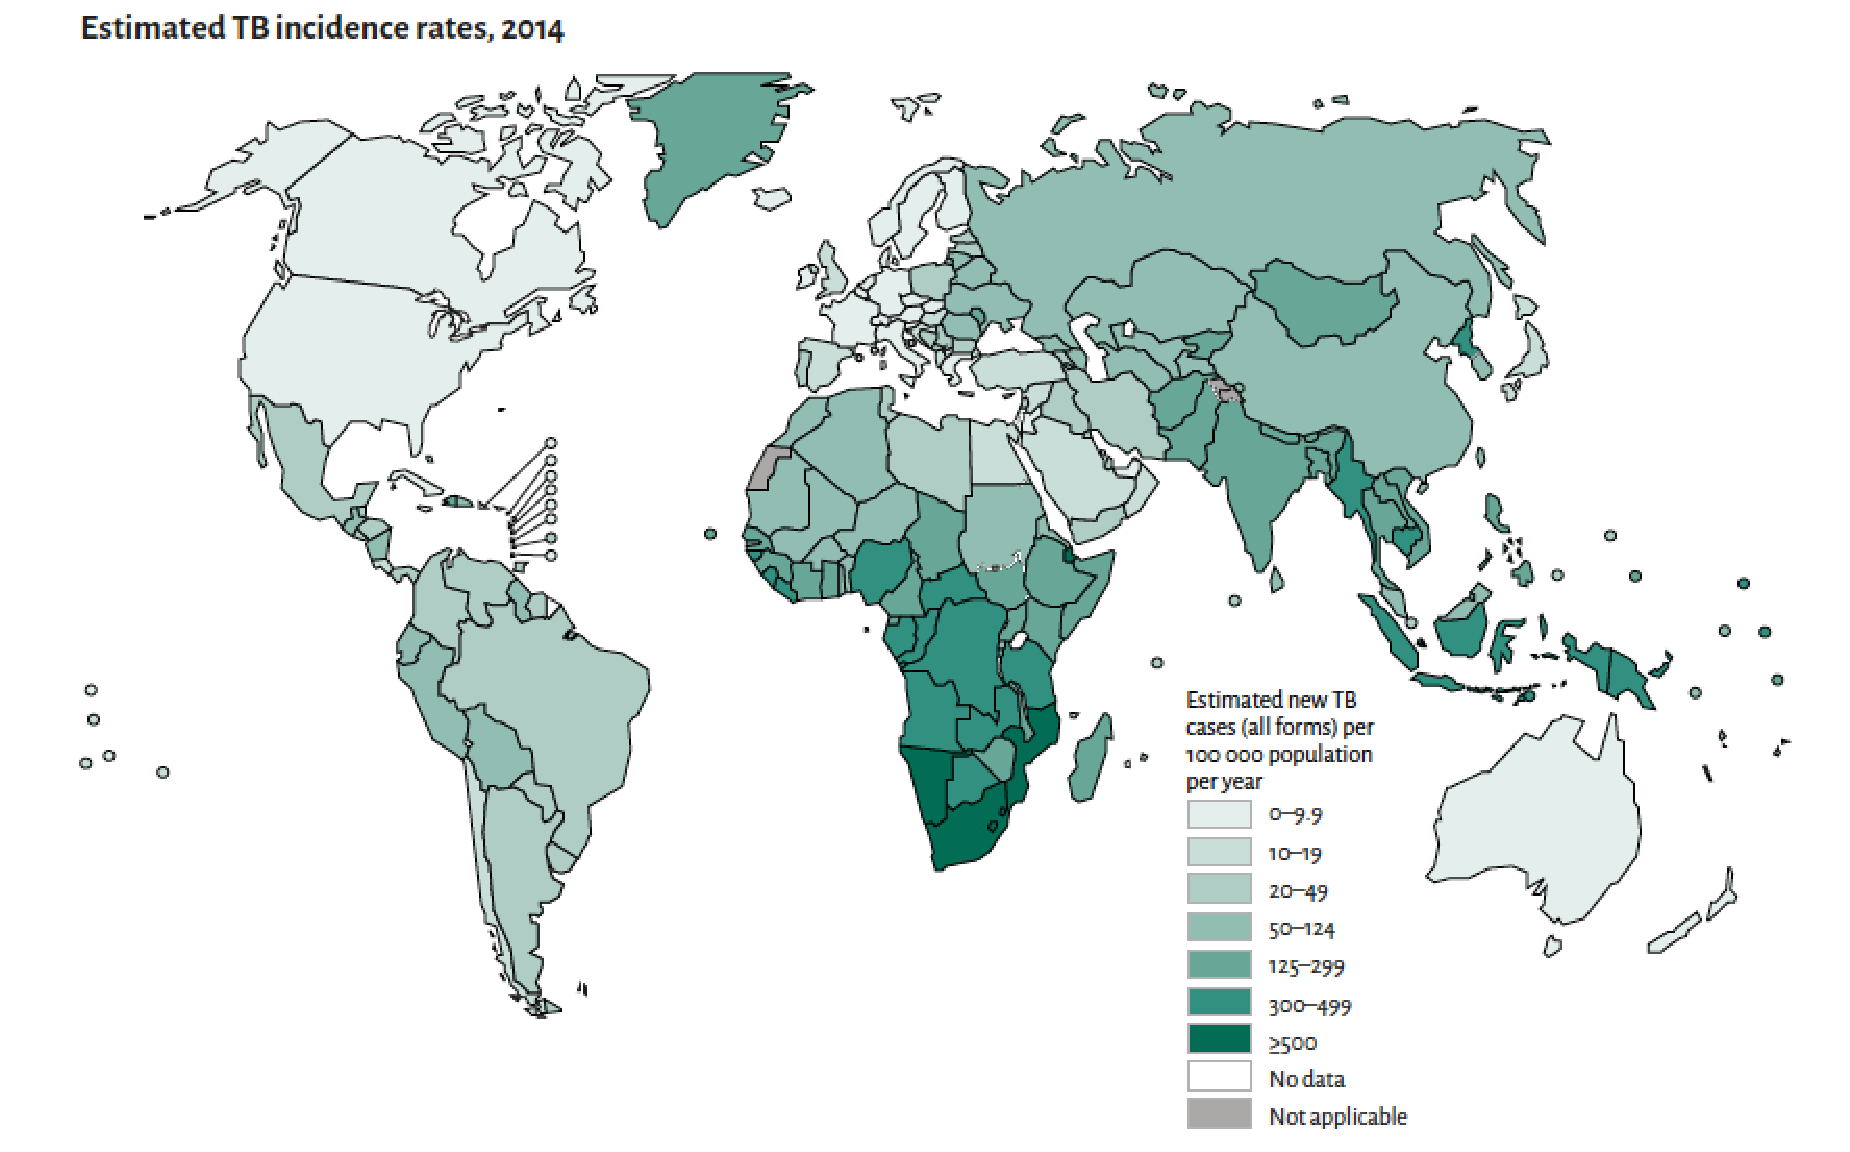
\includegraphics[width=0.9\linewidth]{../figures/map_incidence_tb.pdf}
	\caption{Estimated worldwide TB incidence rates in 2014. Figure extracted from \cite{Lewandowski2015}.}
\label{fig:map_incidence_tb}
	
	\vspace*{4mm}
\end{figure}

\par These strategies are essentially created to bridge the financing gap in Tuberculosis R$\&$. The section will be focused on specific methodologies and tools applied to perform research in this disease. Particular attention will be given to computer aided strategies applied to the TB research and discovery field. 

\subsection{Research strategies against MTB.}\label{mtb_research}

\par Beyond the funding problems of research against MTB, there are numerous technical challenges in identifying new antitubercular compounds \cite{Zuniga2015}. One the main difficulties is the extremely slow growth rate of \textit{Mycobacterium tuberculosis} as this is ultimately reflected in the rate of progress of discovery research. Another aspect is associated which the nature of the bacteria; MTB is a respiratory pathogen, and therefore has to be handled under strict safety conditions (Bio-safety Level 3) requiring expensive specialist facilities. MTB have a very unusual cell wall that impedes many compounds from penetrating into the cell \cite{Brennan2003}. Additionally, this bacteria has efflux pumps that transport compounds out of the cell and that have been implicated in resistance to antibiotics \cite{Rodrigues2012}. Another problem, consequence of the long-term therapy required to treat TB, is that anti-tubercular drugs need to be safe for periods over 6 months (or even more when dealing with MDR-TB or XDR-TB), without significant side effects or drug-drug interactions. [AQUI]
\par The search for new anti-tubercular is therefore a challenging task. Currently, researchers are employing many different approaches in parallel including HTS and computational methods. Such screenings aim to find new molecular entities that could lead to the development of new antibacterial treatments. One of these HTS approaches is the \textit{cell based phenotypic screening}, which represents a powerful approach to identify anti-bacterial compounds and elucidate novel targets \cite{Manjunatha2015}. Some phenotypic screenings are combined with toxicity assays to find those compounds with high anti-tubercular activity and good PK profile \cite{Ballell2013}. Other HTS approaches aim to identity highly potent molecules against a essential MTB target \cite{Park2015, Arora2014}.  Computational methods are essential in the analysis of the vast amount of data generated by HTS and provide a very powerful tool to identity those candidate molecules that could be prioritized for further development. 

\subsubsection{In-silico approaches in TB}

\par Similarly to many other diseases, CADD methods play a substantial role in the Tuberculosis R$\&$ field. Uncountable \textit{in-silico} methods have been published over the last decade \cite{Ekins2013}, each of them applying different strategies to solve a specific bio-medical question. However, all of them pursue the very same goal: fueling drug discovery against TB. Table \ref{table_mtb_methods} contains some remarkable \textit{in-silico} resources for the fight
against TB. The purpose of these resources is very diverse. One popular resource is targetTB, which consist on an open-source pipeline to identify targets in MTB \cite{Raman2008}. Similarly, chapter [REF OUT CHAPTER] presents how the combination of three orthogonal approaches can help to identify the molecular targets of new anti-tubercular compounds. Other resources go beyond a computational pipeline and join a target detection tool with a database of known existing targets and anti-microbial compounds, such is the case of TDRtargets \cite{Crowther2010} (\url{http://tdrtargets.org/}) and CCD-TB \cite{Ekins2010} . Other resources, on the other hand,  are focused on provide specific insights about particular  Most of these resources take advantage of Tuberculist and TuberQ, two databases that include data respectively. Finally, TB-Mobile.  
\renewcommand{\arraystretch}{1.2} %<- modify value to suit your needs
\begin{table}[h!]
 \centering

 \begin{tabular}{*{4}{|| p{3cm} | p{1.85cm}  |  p{5cm} | p{2cm}} ||} 
 \hline
 \tr\textbf{Type of method}\br &\tr\textbf{Name}\br  & \tr\textbf{Resource description}\br & \tr\textbf{Reference(s)}\br\\  
\hline
 Target identification pipeline & TargetTB & Target prioritization in TB thorough a computational pipeline   & \cite{Raman2008}  \\ 
 \hline
 Database &  TDRtargets & Database and method for identification of potential MTB targets & \cite{Crowther2010} \\
 \hline   
 Application of bioinformatics tools & -  & Drug repositioning applied to MDR-TB and XDR-TB & \cite{Kinnings2009}  \\
 \hline
  Database &  CDD-TB & Database of anti-tubercular compounds reported from HTS alongside computational models to analyze the data  &   \cite{Ekins2010}  \\
 \hline
 Application of bioinformatics and chemoinformatics tools & -  & Identification of the MTB targets of bio-active anti-tubercular compounds using three orthogonal \textit{in-silico } approaches & \cite{Martinez-Jimenez2013, Rebollo-Lopez2015}   \\ 
 \hline
  Application of bioinformatics tools &  -  & Homology modelling and virtual doking applied to ligand-protein interaction prediction & \cite{DeJonge2007} \\
 \hline
 Application of chemoinfomatics tools & TB Mobile &   Mobile app that provides a platform to interact with data collected from CDD-TB & \cite{Ekins2013, Clark2014} \\
 \hline 

     Application of bioinformatics and chemoinformatics tools & - & Identification of Enoyl acyl carrier protein reductase binders using a 3D-QSAR approach & \cite{Kumar2009} \\
   \hline
    Application of bioinformatics tools & - &  Interactome computational analysis to identify potential mechanisms of drug resistance to TB therapies & \cite{Raman2008} \\
   \hline
    Database & Tuberculist &  Database of experimentally measured gene essentiality & \cite{Lew2011} \\
   \hline
    Database & TuberQ &  MTB protein druggability database  &  \cite{Radusky2014} \\
   \hline
  
\end{tabular}

\label{table:table_mtb_methods}
\caption{Table containing multiple computational resources used in the discovery and research against TB}
\end{table}







\section{Targeted cancer therapies}

\par Cancer is one the leading causes of morbidity and mortality worldwide. In 2012 there were more than 14 million new cases and 8.2 million cancer related deaths. Moreover, the cancer global burden is expected to rise by about 70$\%$ over the next 20 years \cite{WHO_CANCER}. Intravenous cytotoxic chemotherapy has traditionally prevailed as the main therapeutic choice in cancer treatment. Chemotherapy drugs target rapidly dividing cells, including cancer cells and certain normal tissues.  Hence, the lack of specificity of the chemotherapy treatment leads to strong side side effects such as hair loss, gastrointestinal symptoms, fatigue or myelosuppression, among others.  In the past decade, however, the arrival of targeted cancer therapies have dramatically transformed cancer treatment. Targeted cancer therapies are drugs designed to specifically interfere with molecules necessary for tumorigenesis. The higher specificity associated to these drugs makes them a more powerful and less harming alternative for cancer treatment. Although chemotherapy remains the treatment of choice for many malignancies, targeted therapies are now a essential component of treatment for many types of cancer, including breast, colorectal, non-small cell lung cancer (NSCLC), as well as lymphoma, several classes of leukemia, and multiple myeloma.There are two main types of targeted cancer therapies:  monoclonal antibodies and small molecule inhibitors.

\subsection{Monoclonal antibodies}

\par  Monoclonal antibody-based therapy for cancer has become established over the past 15 years. Additionally, it is currently one of the most successful and promising approaches for treating cancer patients. Monoclonal antibodies are target specific, which means that they exclusively target only one protein. Moreover, their protein target has to be extra cellular, as the antibodies cannot enter the cell through the plasma membrane. Monoclonal antibodies can kill tumour cells throughout multiple mechanism of action \cite{Scott2012}. One of the classic mechanism consist on direct action of the antibody on the target protein. An example of this class is the monoclonal antibody cetuximab, an epidermal growth factor receptor (EGFR) inhibitor used in EGFR-positive colorectal cancer \cite{Jonker2007} and squamous cell carcinoma of the head and neck (SCCHN) \cite{Tejani2010}. Another mechanism consist on the activation of the immune system response to kill cancer cells. Immunotherapies are becoming increasingly popular and its currently one of the most promising fields of cancer research.  Examples of this class include the immune checkpoint inhibitors  pembrolizumab (PD-1), atezolizumab (PDL-1) and ipilimumab (CTLA-4) \cite{Postow2015}; or the CD52 antibody alemtuzumab \cite{Demko2008}. Tumour vascularization and stroma have also been targeted by antibody-based therapies. For example, bevacizumab, is a monoclonal antibody that blocks angiogenesis by targeting the vascular endothelial growth factor receptor (VEGFR) \cite{Ferrara2004}. It is currently used as a single agent or in combination with chemotherapy to treat certain types of advanced cancer, including colorectal, NSCLC, glioblastoma or kidney cancer \cite{Keating2014}. Finally, several conjugated antibodies have been approved to treat cancer. An example of this class is ibritumomab tiuxetan, a yttrium-90-conjugated monoclonal antibody to CD20, for patients with relapsed B-cell non-Hodgkin's lymphomas. This drug combines the monoclonal antibody ibritumomab in conjunction with the chelator tiuxetan, to which radioactive isotope is added \cite{Witzig2002}. Undoubtedly, antibody-based cancer therapies have significantly contributed to the improvement of cancer survival. However, these therapies have still important limitations which prevents them for broader application. One the major limitations is the temporally efficacy of some treatments. Patients with malignant tumours may not achieve a long-term therapeutic effect consequence of the multiple tumour escape mechanisms \cite{Scott2012}. Deeper understanding of the tumor biology may provide insight into selection of patients who are suited to a specific antibody treatment. In summary, monoclonal antibodies has shown a great potential in the treatment of cancer. However, there are important limitations that need to be addressed in order to increase the clinical impact of this type of treatment.  

\subsection{Small molecule kinase inhibitors}

\par Small molecule inhibitors is the second main class of targeted cancer therapies.  Unlike monoclonal antibodies, they can penetrate into the cell throughout the plasma membrane. Small molecule targeted cancer therapies focus on inhibiting protein kinases. In fact, kinases have been established as promising drug targets for the treatment of various types of human disease because of their essential roles in signal transductions and regulation of a range of cellular activities. However, the vast majority of these targets are being investigated for the treatment of cancer \cite{Zhang2009}.  Over the last years,  many kinases have been found to be deeply involved in the processes leading to tumorigenesis. Depending of their role in cancer progression we can classify small molecule kinase targets into different groups.  First, there are kinases that have become insensitive to normal regulatory mechanisms. The altered activity of such kinases can be the consequence of genetic alterations (e.g. mutations or translocations) or epigenetic changes (e.g. gene amplification, increased expression) and are considered to be oncogenic. The constitutive activity of this class of kinase target makes them essential for survival and/or proliferation of the cancer cell. This phenomenon is known as oncogene addiction \cite{Weinstein2006}, and makes the cancer cell exceptionally susceptible to the oncogene kinase inhibitor. One of best examples of this phenomenon is the activating V600E BRAF mutation. About 50 $\%$ of melanomas harbour this oncogenic mutation \cite{Ascierto2012}. Currently, there are two small molecules FDA approved inhibitors (vemurafenib \cite{Bollag2010} and dabrafenib \cite{Gibney2013}) that specifically target the BRAF V600E-mutated metastatic melanoma. Inhibiting mutationally activated kinases (i.e., oncogenic kinases) has resulted in the most dramatic clinical responses \cite{Zhang2009}.  A second class of target kinases is composed by those non-oncogenic kinases whose presence is preferentially required for the survival and/or proliferation of tumour cells.  These kinases are usually located in key signalling pathways downstream of cancer oncogenes. Examples of this type of targets include MEK1 and MEK2 (also known as MAP2K1 and MAP2K2), which are targeted by several small molecule inhibitors such as trametinib or cobimetinib. Combinations of these inhibitors with oncogene inhibitors led into a significant improvement in patient survival compared with single treatment regime in melanoma \cite{Flaherty2012, Flaherty2012a}. Another class of kinases targets are those highly expressed in the tumour stroma and that are required for different stages of tumour formation and development in the human host. Examples of this class include the inhibition of VEGFR by pazopanib or other small molecule inhibitors \cite{Ivy2009}. Kinase targets of the second and third classes are not directly oncogenic, but instead are required for the survival and proliferation of cancer cells. Hence, the inhibition of these kinases is usually combined with oncogene inhibition to strengthen the inhibitory effect and overcome resistance due to activation of downstream survival mechanisms \cite{Holohan2013}. 
 
 \par Protein kinases are defined by their ability to catalyse the transfer of the terminal phosphate of ATP to a substrate that usually contains a serine, threonine or tyrosine.  They share a highly conserved arrangement of secondary structure elements that fold into a bi-lobed catalytic core structure, with ATP binding site located in a deep cleft located between the two lobes \cite{Manning2002}. The ATP adenine ring forms hydrogen bonds with the kinase hinge region (i.e., the segment that connects the amino and carboxy terminal kinase domains , FIGURE), while the ribose and triphosphate groups of ATP bind in a hydrophilic channel extending to the ATP binding site that contains conserved residues that are essential to catalysis. Additionally, kinases have a conserved activation loop, which regulates the kinase activity that contains a extremely conserved DFG (i.e., aspartic acid, phenylalanine and glycine) motif at the start of the loop (Figure). The structural disposition of the activation loop switches between active and inactive conformations of the protein kinase \cite{Manning2002}. Therefore, selective targeting of a kinase in the active state using conventional ATP-compatitive inhibitors is innately challenging. In contrast, kinase inactive states are structurally highly diverse and dynamic, suggesting that inhibitors targeting such states should have a better chance of being selective \cite{Muller2015}. POR AQUI
 
 Most of the current small molecule kinase inhibitors are ATP-competitive that mimics the ATP binding mode. Concretely,    
 Depending on their biochemical mode of action, small molecule protein kinase inhibitors can be classified multiple classes
 On the basis of their binding modes, kinase inhibitors have been categorized as type I inhibitors that bind the active state
 Problem of multitarget!!! 
 Since the catalytic mechanism requires the exact positioning of highly conserved active site residues, the kinase active state is rigid and highly conserved. Therefore, selective targeting of a kinase in the active state using conventional ATP-compatitive inhibitors is innately challenging. In contrast, kinase inactive states are structurally highly diverse and dynamic, suggesting that inhibitors targeting such states should have a better chance being selective.( Muller2015)
 
 
 
  


\par complete list. 


\subsection{Resistance to targeted cancer therapies}





\chapter{Objectives}

\chapter{nAnnolyze}
\chapter{Predicting targets in MTB}
\chapter{Drug resistance in cancer}



\begin{figure}[b]
  \centering
  
\includegraphics[scale=0.5]{../figures/logo_upf.png}
    \caption{Example}
    \label{fig:logo}
\end{figure}





%\bibliography{/Users/fran/Documents/Work/tesis/bibliography/bibliography_tesis}



\backmatter
\printindex

\printbibliography






\end{document}
